% !TEX root = ./rosbook_jp.tex
%-------------------------------------------------------------------------------
\chapterimage{chapter_head_11.pdf}

%-------------------------------------------------------------------------------
\chapter{ROSによるロボットアームの制御}\index{ROSによるロボットアームの制御}

本章では、ROSが提供する様々なパッケージを利用して、ロボットアームを制御する方法について説明する。最初に一般的なロボットアームの構成について解説した後、ROSで一般的に用いられるロボット表記法であるURDF形式について、簡単な3関節ロボットアームとタートルロボットアームを例に説明する。その後、ロボットアームの動作計画パッケージであるMoveItについて、把持動作の計画方法や実際のロボットアームを用いた使用法を紹介する。

%-------------------------------------------------------------------------------
\section{ロボットアームとは}\index{ロボットアームとは}

 ロボットアームは,電気や油圧で駆動する関節を持つ腕型のロボットであり、マニピュレータとも呼ばれる。現在、ロボットアームは、組立、溶接、塗装、移送作業など、高精度の繰り返し動作が求められる作業現場や、危険、あるいは人手では困難な作業を伴う現場で広く利用されている。特に、単純だが危険を伴う自動車の溶接・塗装工程や、高い精度と信頼性を必要とする半導体組み立て工程などでは欠かせないものとなっている。
また、ロボットアームは、産業用ロボットだけでなく、ヒューマノイドロボットやサービスロボットの腕としても広く使用されている。例えば、9章で紹介したタートルボットはロボットアームを搭載でき、アームを使って床面上の物品の把持や搬送が可能となる。

%-------------------------------------------------------------------------------
\section{ロボットアームの構成要素と種類}\index{ロボットアームの構成要素と種類}

ロボットアームを構成する要素は、図11-1に示すように、リンク(link)、関節(joint)、エンドエフェクタ(end effector)の3種類に分けられる。ロボットアームの一端は、土台部分であるベース(base)に固定されている。産業用ロボットでは、ロボットはベースである床面に固定されるが、移動ロボットに取り付けられたロボットアームのように、ベースが移動可能な場合もある。エンドエフェクタは、リンクと関節を腕と見立てた場合、手に対応する部分であり、物体把持や様々な作業に使われる。


\begin{figure}[htp]
  \centering
  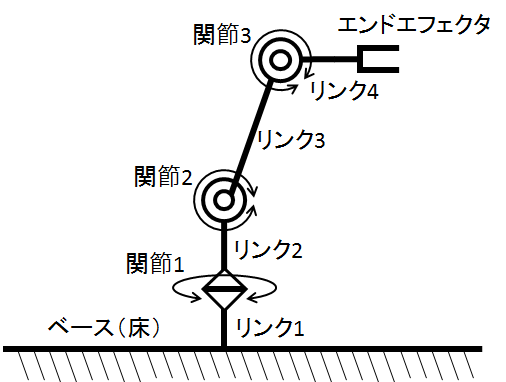
\includegraphics[width=10cm]{pictures/chapter11/pic_11_01.png}
  \caption{3関節ロボットアームの構成要素}
\end{figure}

リンクは、ベース、関節、エンドエフェクタをつなぐ剛体部品である。関節は、モータや油空圧アクチュエータによる駆動部分で、軸回りに回転する回転運動型、ある方向に並進運動する直動運動型に分けられる。エンドエフェクタにはさまざまな種類があり、作業目的に応じたものを選択・装着する。例えば塗装で使用されるスプレーガン、溶接トーチ、ドリル、グラインダーなどのツールや、あるいは物体を把持するグリッパーや多指ハンドなどがある。
ロボットアームは、関節の種類や配置によって、極座標型、円筒座標型、直交座標型、水平多関節型、垂直多関節型などに分けることができる。サービスロボットの多くは、図11-2のような人間の腕に最も近い垂直多関節型ロボットアームである。

\begin{figure}[htp]
  \centering
  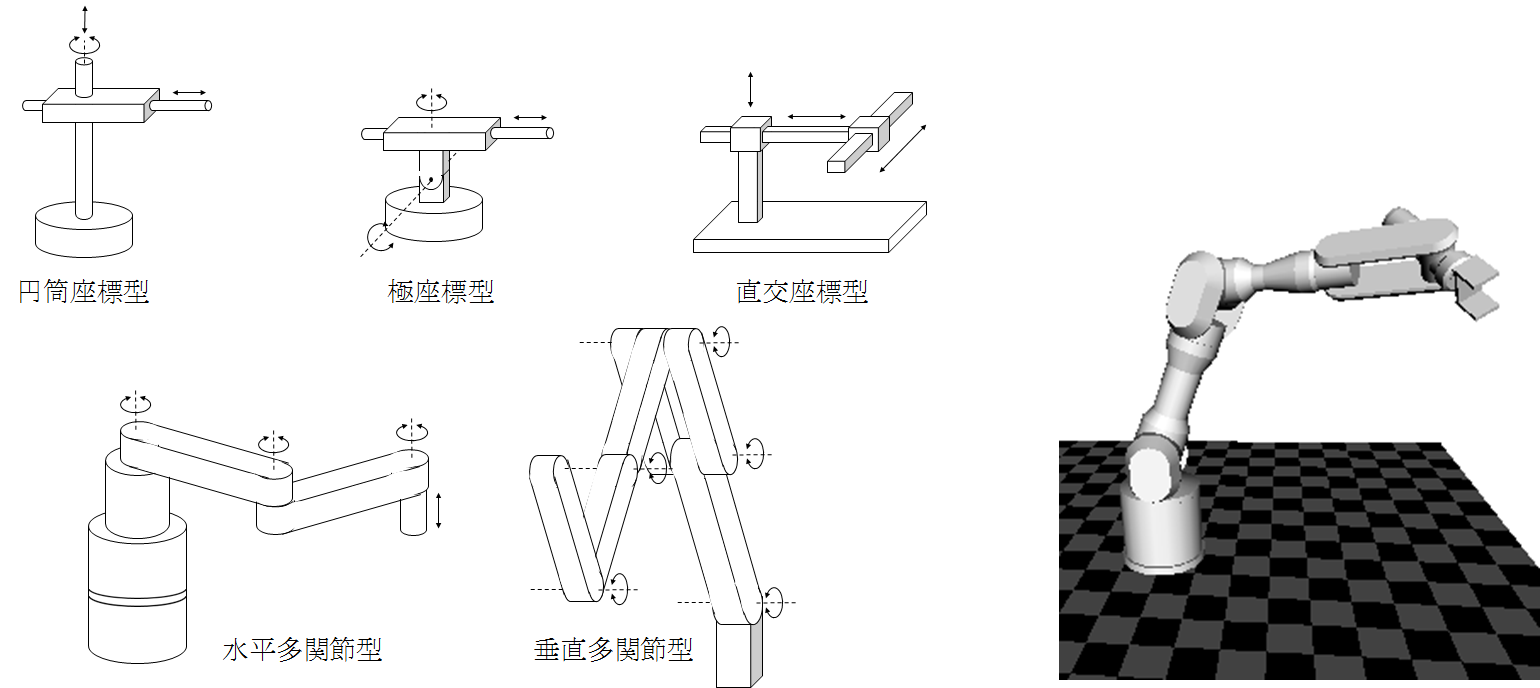
\includegraphics[width=12cm]{pictures/chapter11/pic_11_02.png}
  \caption{ロボットアームの分類と垂直多関節型マニピュレータ}
\end{figure}

%-------------------------------------------------------------------------------
\section{ロボットアームの動作計画}\index{ロボットアームの動作計画}

ロボットアームで、ある場所に置かれた既知の物体を把持し、目的の場所まで運び、置く作業(ピック&プレイス)を考える。最も簡単な方法は、物体を把持するときの各関節の角度や、目的の場所に置くときの各関節の角度をあらかじめ求めておき、作業時には各関節がその角度になるように関節を一斉に動かすことである。しかし、この方法は、把持しようとした物体の大きさや形状、物体の設置場所、把持位置が変更されると適用できない。また、把持位置と設置位置の間に障害物が存在した場合、それを回避できない。
そこでロボットアームによるピック&プレイスの制御には、物体の大きさや形状、設置位置に応じた把持位置の設定や、障害物との衝突を回避する動作計画などの機能が必要である。ROSでは、これらの機能をMoveIt注1というモーションプランニングパッケージで提供する。MoveItを利用するうえで、ロボットアームに関する深い知識は必ずしも必要なく、上記の機能は比較的簡単に実現できる。ただし、基本的な知識や理解はもっておくべきであり、本節ではその説明を行う。

\subsubsection{作業空間と関節空間}

ロボットアームの制御において、「作業空間」と「関節空間」という2つの概念は非常に重要である。まずはこれらを理解しよう。
XYZ座標系などで定義された3次元空間で、ロボットに作業命令を与える状況を想定する。例えば、「そこの物を取れ」という命令を与えるとき、実際には「そこ」は3次元空間内のある(x,y,z)座標点で表す。ロボットアームがこの命令を実行するには、手先が指示された座標に来るように、自身の関節を適切に動かさなければならない。したがって、ロボットアームにとって必要な情報は、各関節の回転角度である。つまり、私たちが与える情報とロボットが動作に必要な情報は異なる。
ここで、ロボットアームが動作する3次元空間は、ロボットの手に対応するエンドエフェクタの位置と姿勢で表現できる。3次元空間では、位置は(x,\ y,\ z)の3つの変数で、姿勢はx軸、y軸、z軸回りの角度である(θ,φ,ψ)の3つの変数で記述できる。これをまとめた6つの変数(x,\ y,\ z,θ,φ,ψ)で表わされる空間を作業空間(Work Space)という。一方で、ロボットがエンドエフェクタを決められた位置、姿勢へ動かすには、各関節の角度(θ1,θ2,θ3,...)の適切な値を計算しなければならない。この関節の角度を表す空間を関節空間(Joint Space)という。

\subsubsection{自由度}

もうひとつの重要な概念として「自由度」も理解しておこう。自由度(DOF、degrees of freedom)は、ロボットや物体の状態を表現する、最小限の独立した変数の数である。例えば、3次元空間上に置かれている物体の運動は、x、y、z方向の並進運動と、x、y、z軸回りの角度θ、φ、ψの回転運動の6変数を得られれば表現可能であり、すなわち6自由度である。また7つの関節を持つロボットの姿勢は、7つの変数(各関節の角度)で決定できることから、7自由度を有していると言える。ロボットにより、物体の位置と姿勢を同時に独立して変えたいときには、ロボットには物体が持つ自由度(6自由度)以上の自由度が必要である。しかし、もし動きの一部を制限しても作業に支障がないときは、必ずしもロボットに6自由度以上の自由度を持たせる必要はない。

\subsubsection{順運動学と逆運動学}

ロボットを目的通り動作させるためには、まず幾何学的な運動計画を立て(Kinematics、運動学計算)、重力や慣性力などの動力学的な効果を計算して(Dynamics、動力学計算)、それぞれの関節に適切な指令値を与えなければならない。ここで、関節空間でロボットの各関節の角度(直動関節であれば長さ)が与えられたとき、作業空間でのエンドエフェクタの位置および姿勢を求めることを順運動学(FK、Forward Kinematics)計算と呼ぶ。逆に、作業空間でエンドエフェクタの位置と姿勢が与えられたとき、関節空間での各関節の角度を求めることを逆運動学(IK、Inverse Kinematics)計算と呼ぶ。これらの詳細な説明は、ロボット工学関連書籍を参照してほしい。11.5節では、順運動学計算、逆運動学計算にMoveItパッケージを利用し、ロボットアームを制御する方法を説明する。

%-------------------------------------------------------------------------------
\section{ロボットアームのモデリング}\index{ロボットアームのモデリング}

ロボットアームの構成要素であるリンク、関節、エンドエフェクタなどのモデルを記述するために、ROSではURDF注2(Unified Robot Description Format)と呼ばれる形式を利用する。URDFで記述されたロボットモデルは、RVizに直接読み込んで表示できる。さらに、RViz上で各関節を仮想的に動かすことで、設計したモデルが正しいかを確認できる。また、RVizでロボットモデルを読み込み、各関節の値を入力すれば、実際のロボットを動作させることもできる。また作成したモデルは、MoveItによる動作計画や、Gazeboシミュレータによる動力学シミュレーションに用いることもできる。以降では、これらの一連の手順を紹介する。

%-------------------------------------------------------------------------------
\subsection{3関節ロボットアームのモデリング}

前述のように、ROSはURDF形式でロボットアームの各構成要素を記述する。URDF形式では、最初にロボットの名前、ベースの名前や種類、ベースが接続しているリンクを記述し、続いてリンクや関節の詳細を一つずつ記述する。リンクについては、リンクの名前や大きさ、重さや慣性などを記述する。また関節については、関節の名前、種類、各関節が接続しているリンクを記述する。
実際に、図11-3のような4つのリンクと3つの関節からなるロボットアームをモデル化してみよう。次のようにtestbot\_descriptionというパッケージを作成した後、urdfという名前のフォルダを作成する。次に、エディタを使用して、testbot.urdfという名前のファイルを作成して、以下のURDFの例を入力しよう。

\begin{lstlisting}[language=ROS]
$ cd ~/catkin_ws/src
$ catkin_create_pkg testbot_description urdf
$ cd testbot_description
$ mkdir urdf
$ cd urdf
$ gedit testbot.urdf
\end{lstlisting}

\textbf{ファイル名:testbot.urdf}
\begin{lstlisting}[language=XML]
<?xml version="1.0" ?>
<robot name="test_robot">

  <material name="black">
    <color rgba="0.0 0.0 0.0 1.0"/>
  </material>
  <material name="orange">
    <color rgba="1.0 0.4 0.0 1.0"/>
  </material>

  <link name="base"/>
  <joint name="fixed" type="fixed">
    <parent link="base"/>
    <child link="link1"/>
  </joint>

  <!-- Link 1 -->
  <link name="link1">
    <collision>
      <origin rpy="0 0 0" xyz="0 0 0.25"/>
      <geometry>
        <box size="0.1 0.1 0.5"/>
      </geometry>
    </collision>
    <visual>
      <origin rpy="0 0 0" xyz="0 0 0.25"/>
      <geometry>
        <box size="0.1 0.1 0.5"/>
      </geometry>
      <material name="black"/>
    </visual>
    <inertial>
      <origin rpy="0 0 0" xyz="0 0 0.25"/>
      <mass value="1"/>
      <inertia ixx="1.0" ixy="0.0" ixz="0.0" iyy="1.0" iyz="0.0" izz="1.0"/>
    </inertial>
  </link>
  <joint name="joint1" type="revolute">
    <parent link="link1"/>
    <child link="link2"/>
    <origin rpy="0 0 0" xyz="0 0 0.5"/>
    <axis xyz="0 0 1"/>
    <limit effort="30" lower="-2.617" upper="2.617" velocity="1.571"/>
  </joint>

  <!-- Link 2 -->
  <link name="link2">
    <collision>
      <origin rpy="0 0 0" xyz="0 0 0.25"/>
      <geometry>
        <box size="0.1 0.1 0.5"/>
      </geometry>
    </collision>
    <visual>
      <origin rpy="0 0 0" xyz="0 0 0.25"/>
      <geometry>
        <box size="0.1 0.1 0.5"/>
      </geometry>
      <material name="orange"/>
    </visual>
    <inertial>
      <origin rpy="0 0 0" xyz="0 0 0.25"/>
      <mass value="1"/>
      <inertia ixx="1.0" ixy="0.0" ixz="0.0" iyy="1.0" iyz="0.0" izz="1.0"/>
    </inertial>
  </link>
  <joint name="joint2" type="revolute">
    <parent link="link2"/>
    <child link="link3"/>
    <origin rpy="0 0 0" xyz="0 0 0.5"/>
    <axis xyz="0 1 0"/>
    <limit effort="30" lower="-2.617" upper="2.617" velocity="1.571"/>
  </joint>

  <!-- Middle Link -->
  <link name="link3">
    <collision>
      <origin rpy="0 0 0" xyz="0 0 0.5"/>
      <geometry>
        <box size="0.1 0.1 1"/>
      </geometry>
    </collision>
    <visual>
      <origin rpy="0 0 0" xyz="0 0 0.5"/>
      <geometry>
        <box size="0.1 0.1 1"/>
      </geometry>
      <material name="black"/>
    </visual>
    <inertial>
      <origin rpy="0 0 0" xyz="0 0 0.5"/>
      <mass value="1"/>
      <inertia ixx="1.0" ixy="0.0" ixz="0.0" iyy="1.0" iyz="0.0" izz="1.0"/>
    </inertial>
  </link>
  <joint name="joint3" type="revolute">
    <parent link="link3"/>
    <child link="link4"/>
    <origin rpy="0 0 0" xyz="0 0 1.0"/>
    <axis xyz="0 1 0"/>
    <limit effort="30" lower="-2.617" upper="2.617" velocity="1.571"/>
  </joint>

  <!-- Top Link -->
  <link name="link4">
    <collision>
      <origin rpy="0 0 0" xyz="0 0 0.25"/>
      <geometry>
        <box size="0.1 0.1 0.5"/>
      </geometry>
    </collision>
    <visual>
      <origin rpy="0 0 0" xyz="0 0 0.25"/>
      <geometry>
        <box size="0.1 0.1 0.5"/>
      </geometry>
      <material name="orange"/>
    </visual>
    <inertial>
      <origin rpy="0 0 0" xyz="0 0 0.25"/>
      <mass value="1"/>
      <inertia ixx="1.0" ixy="0.0" ixz="0.0" iyy="1.0" iyz="0.0" izz="1.0"/>
    </inertial>
  </link>

</robot>
\end{lstlisting}

上のURDFファイルは、material、link、jointなどのタグによって構成されている。以下で、各タグについて説明する。

\subsubsection{material}

materialタグには、リンクの色やテクスチャなどの情報を記述する。次の例では、各リンクを区別するために、黒とオレンジ色の二つの材質を定義した。色はcolorタグの後の rgbaオプションの後に、赤、緑、青に対応する0から1の数値をそれぞれ記入することで変更できる。最後の数字は透明度(アルファ)を表すが、通常は使われない。

\begin{lstlisting}[language=XML]
<material name="black">
  <color rgba="0.0 0.0 0.0 1.0"/>
</material>
<material name="orange">
  <color rgba="1.0 0.4 0.0 1.0"/>
</material>
\end{lstlisting}

\subsubsection{link}

linkタグは、それぞれのリンクの特性を記述する。ベースはURDFではリンクの一種として分類されるので、まずはベースを記述する。次の例では、最初の行でbaseという名前のベースをリンクとして宣言している。次のjointタグについては、次頁以降で詳しく説明するが、ここではtypeをfixedとした。これは、ベースとリンク(ベースに接続されるリンクをlink1とする)が固定されていることを示している。

\begin{lstlisting}[language=XML]
<link name="base"/>

<joint name="fixed" type="fixed">
  <parent link="base"/>
  <child link="link1"/>
</joint>
\end{lstlisting}

次は、リンク1の記述例である。

\begin{lstlisting}[language=XML]
<!-- Link 1 -->
<link name="link1">
  <collision>
    <origin rpy="0 0 0" xyz="0 0 0.25"/>
    <geometry>
      <box size="0.1 0.1 0.5"/>
    </geometry>
  </collision>
  <visual>
    <origin rpy="0 0 0" xyz="0 0 0.25"/>
    <geometry>
      <box size="0.1 0.1 0.5"/>
    </geometry>
    <material name="black"/>
  </visual>
  <inertial>
    <origin rpy="0 0 0" xyz="0 0 0.25"/>
    <mass value="1"/>
    <inertia ixx="1.0" ixy="0.0" ixz="0.0" iyy="1.0" iyz="0.0" izz="1.0"/>
  </inertial>
</link>
\end{lstlisting}

このように、リンク1は、collision、visual、inertialタグで構成されている。collisio\\nタグには、リンクの干渉範囲を表す幾何的な情報を入力する。originには、干渉範囲の中心座標を記す。またgeometryには、originを中心とする干渉範囲の形状と大きさを記す。例えば四角柱 (box) 型の干渉範囲では、その縦、横、高さの値である。四角柱型以外にも、円筒型、球型などがあるが、それぞれ入力する内容が異なる。visualタグには、実際の形状を記す。originやgeometryはcollisionタグと同様である。また、ここにSTLやDAEなどのCADファイルを入力することもできる。なお、collisionタグでもCADモデルを使用できるが、ODEやBulletなど一部の物理エンジンでのみ使用でき、DARTやSimbodyなどではサポートしていない。inertialタグには、リンクの重量(mass、単位はkg)と慣性モーメント(moments of inertia、単位はkgm2)を記入する。これらの情報は、動力学シミュレーション時に使用する。
testbot.urdfに記述されたリンク1、リンク2、リンク4は、一方の端を原点とし、z軸方向に伸びた長さ0.5、幅0.1、奥行き0.1の四角柱であり、リンク3も同様に原点からz軸方向に伸びた、長さ1、幅0.1、奥行き0.1の四角柱である。

\begin{figure}[htp]
  \centering
  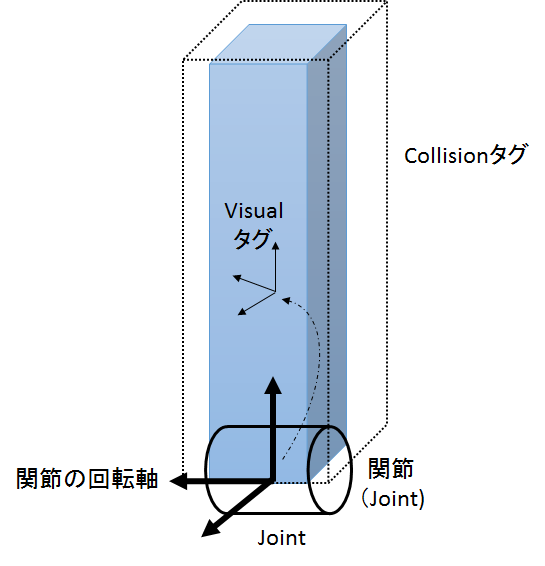
\includegraphics[width=12cm]{pictures/chapter11/pic_11_03.png}
  \caption{リンクの各要素とジョイント}
\end{figure}

\subsubsection{joint}

jointタグは、関節の特性を記述する。具体的には、関節の名前、種類(revolute(回転運動型)、prismatic(直動運動型)、fixed(固定型)など)、接続する2つのリンクの名前、関節の位置、回転および並進運動の基準軸、動作の制限を記述する。接続するリンクには、親リンク、子リンクの名前を指定する。通常、ベースに近いリンクを親リンクとする。
図11-4は、図11-2のリンク2からリンク3までを抜き出して描いたものである。この2つのリンクを接続する関節(関節2)を例に、jointタグの記述について説明する。

\begin{lstlisting}[language=XML]
<joint name="joint2" type="revolute">
  <parent link="link2"/>
  <child link="link3"/>
  <origin rpy="0 0 0" xyz="0 0 0.5"/>
  <axis xyz="0 1 0"/>
  <limit effort="30" lower="-2.617" upper="2.617" velocity="1.571"/>
</joint>
\end{lstlisting}

このjoint2では、種類(type)は回転運動型関節のrevolute、親リンク(parent link)はlin\\k2、子リンク(child link)はlink3に設定した。さらに、originには、一つ前の関節(joint1)の座標系から見た、この関節(joint2)の座標系の相対位置、姿勢を指定する。例えば、joint2の座標系の原点は、joint1の座標系のz軸方向に、joint1から0.5だけ離れた位置である。またaxisには回転運動型関節であれば回転軸の方向を、直動運動型関節であれば運動方向を記入する。このjoint2では、y軸回りに回転する関節であることを示している。 limitには、関節動作に関する制限事項を記述し、関節に与えられる力(effort、単位はN)、最大・最小角度(lower、upper、単位はradian)、速度(単位はrad/s)の制限値を設定する。

\begin{figure}[htp]
  \centering
  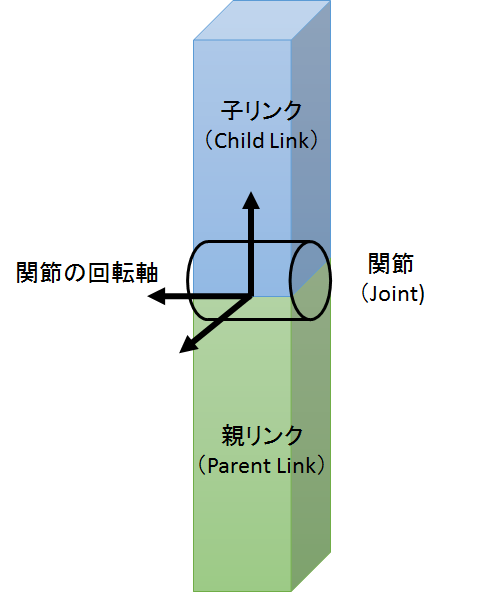
\includegraphics[width=8cm]{pictures/chapter11/pic_11_04.png}
  \caption{関節部分のモデリング要素}
\end{figure}

なお、エンドエフェクタもLink4の先に、linkやjointを組み合わせて作成することができるが、この例では省略している。

\subsubsection{エラーチェック}

モデルの作成が完了したら、作成したURDFに文法の間違いや、リンクや関節のつながりに間違いがないかを確認する。次のコマンドで、liburdfdom-toolsをインストールする。

\begin{lstlisting}[language=ROS]
$ sudo apt-get install liburdfdom-tools
\end{lstlisting}

次に、check\_urdfコマンドで、作成したURDFの文法エラーと各リンクの接続関係が確認する。記述が正しい場合は、次のようにリンク1、2、3、4の接続関係が表示される。これは最初のリンク(root Link)がbaseであり、baseの子リンクがlink1、link1の子リンクがlink2、link2の子リンクがlink3、link3の子リンクがlink4であることを示している。

\begin{lstlisting}[language=ROS]
$ check_urdf testbot.urdf
robot name is: test_robot
---------- Successfully Parsed XML ---------------
root Link: base has 1 child(ren)
child(1):  link1
   child(1):  link2
      child(1):  link3
         child(1):  link4
\end{lstlisting}

記述に間違いがあると、以下の例のようにエラーの詳細が表示される。この例は、link2を削除した場合である。

\begin{lstlisting}[language=ROS]
$ check_urdf testbot.urdf
Error:   Failed to build tree: child link [link2] of joint [joint1] not found
         at line 226 in /build/buildd/urdfdom-0.2.10+dfsg/urdf_parser/src/model.cpp
ERROR: Model Parsing the xml failed
\end{lstlisting}

\subsubsection{グラフ表示}

次に、urdf\_to\_graphizプログラムを利用して、作成されたモデルをグラフで表示する方法を説明する。次の例のように、urdf\_to\_graphizを実行すると、*.gvファイルと.pdfファイルが生成される。これをpdfビューアで表示すると、図11-5のようにlinkとjointが交互に接続されていることが確認できる。

\begin{lstlisting}[language=ROS]
$ urdf_to_graphiz testbot.urdf
Created file test_robot.gv
Created file test_robot.pdf
\end{lstlisting}

\begin{figure}[htp]
  \centering
  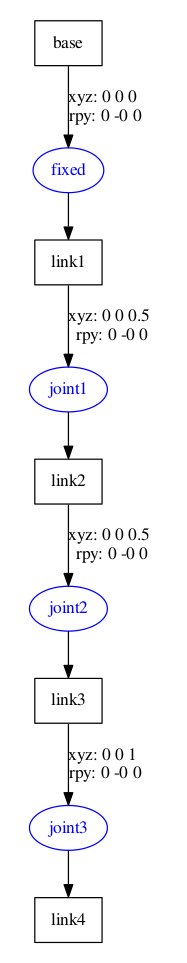
\includegraphics[width=4cm]{pictures/chapter11/pic_11_05.png}
  \caption{URDFのlinkとjointの関係}
\end{figure}

\subsubsection{RVizによるモデルの動作チェック}

上述のように、check\_urdfとurdf\_to\_graphizを用いれば、モデルの文法やリンクや関節のつながりを確認できる。しかし文法や構造には問題がなくても、例えば関節の位置や関節軸の方向、あるいはリンクの長さに誤りがある場合など、望んだ通りのモデルになっているとは限らない。そのため、3次元可視化ツールRVizを利用して、作成されたモデルを表示し、想定通りに作成されているかを確認する必要がある。手順は以下のとおりである。
まず、次のように、testbot\_descriptionパッケージフォルダに移動し、launchフォルダを作成して、そこに移動する。

\begin{lstlisting}[language=ROS]
$ cd ~/catkin_ws/src/testbot_description
$ mkdir launch
$ cd launch
\end{lstlisting}

続いて、エディタを開き、testbot.launchファイルを新たに作成する。

\begin{lstlisting}[language=ROS]
$ gedit testbot.launch
\end{lstlisting}

作成するtestbot.launch ファイルの内容を以下に示す。

\textbf{ファイル名: testbot\_description/launch/testbot.launch}

\begin{lstlisting}[language=XML]
<launch>
  <arg name="model" default="$(find testbot_description)/urdf/testbot.urdf" />
  <arg name="gui" default="True" />
  <param name="robot_description" textfile="$(arg model)" />
  <param name="use_gui" value="$(arg gui)"/>
  <node name="joint_state_publisher" pkg="joint_state_publisher" type="joint_state_publisher" />
  <node name="robot_state_publisher" pkg="robot_state_publisher" type="state_publisher" />
</launch>
\end{lstlisting}

このtestbot.launch ファイルでは、まず上で作成したモデルtestbot.urdfを呼び出し、図11-6のように、joint\_state\_publisherノードがモデルのjoint情報に基づいて関節角度値を配信する。その後、robot\_state\_publisherノードが関節の情報を購読し、配信された関節角度値の変化に応じて各関節とリンクの間の3次元位置、姿勢情報をtfトピックとして配信する。

\begin{figure}[htp]
  \centering
  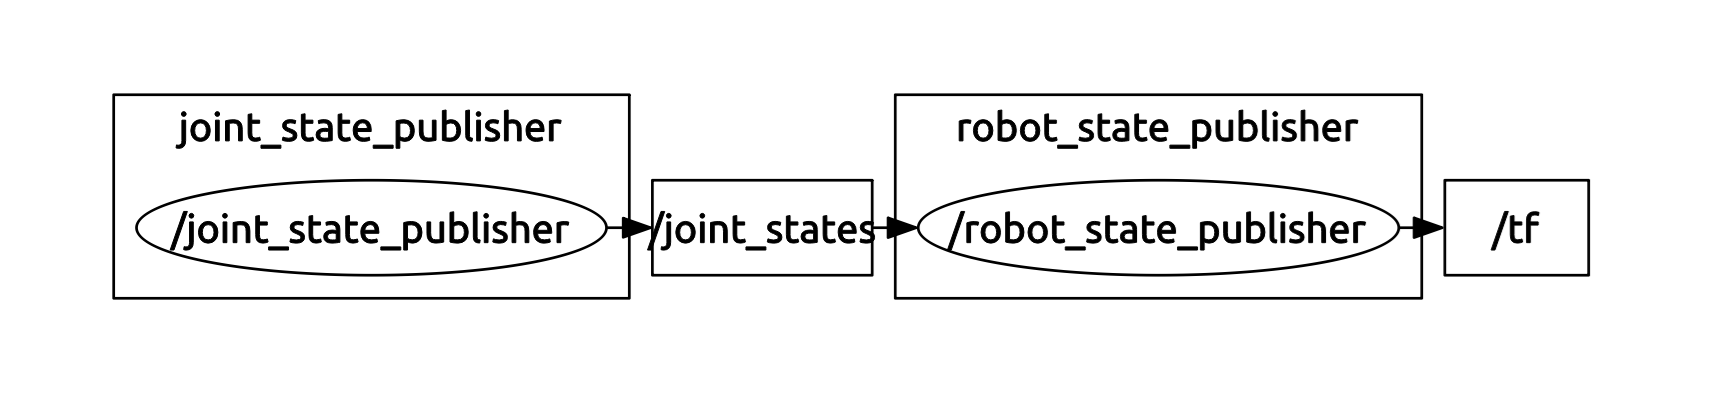
\includegraphics[width=12cm]{pictures/chapter11/pic_11_06.png}
  \caption{joint\_state\_publisherノードとrobot\_state\_publisherノードのトピック通信}
\end{figure}

testbot.launchファイルを作成した後、次のようにtestbot.launchとRVizを実行する。

\begin{lstlisting}[language=ROS]
$ roslaunch testbot_description testbot.launch
$ rosrun rviz rviz
\end{lstlisting}

launchファイルが実行されると、図11-7に示すようなjoint\_state\_publisherノードのGUI画面が現れる。この画面上では、joint 1、2、3の関節値を調整できる。その後、RVizの画面で [Fixed Frame]で「base」を選択し、左下の<Add>ボタンをクリックして「RobotModel」を追加すれば、図11-8のようにRVizで各関節とリンクを表示できる。そして、joint\_state\_publisherノードのGUI画面で各関節のパラメータを変更すると、図11-9のようにRViz上の仮想ロボットが動作する。
本項で作成したtestbot.urdfとtestbot.launchは、githubリポジトリ「https://github.com/irvs/rosbook\_robot\_arm」から入手できる。ダウンロードの方法は以下の通りである。

\begin{lstlisting}[language=ROS]
$ git clone https://github.com/irvs/rosbook_robot_arm.git
\end{lstlisting}

\begin{figure}[htp]
  \centering
  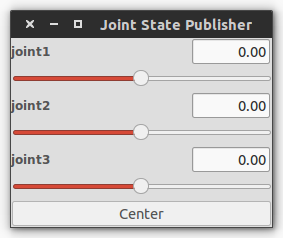
\includegraphics[width=8cm]{pictures/chapter11/pic_11_07.png}
  \caption{Joint State PublisherのGUI画面}
\end{figure}

\begin{figure}[htp]
  \centering
  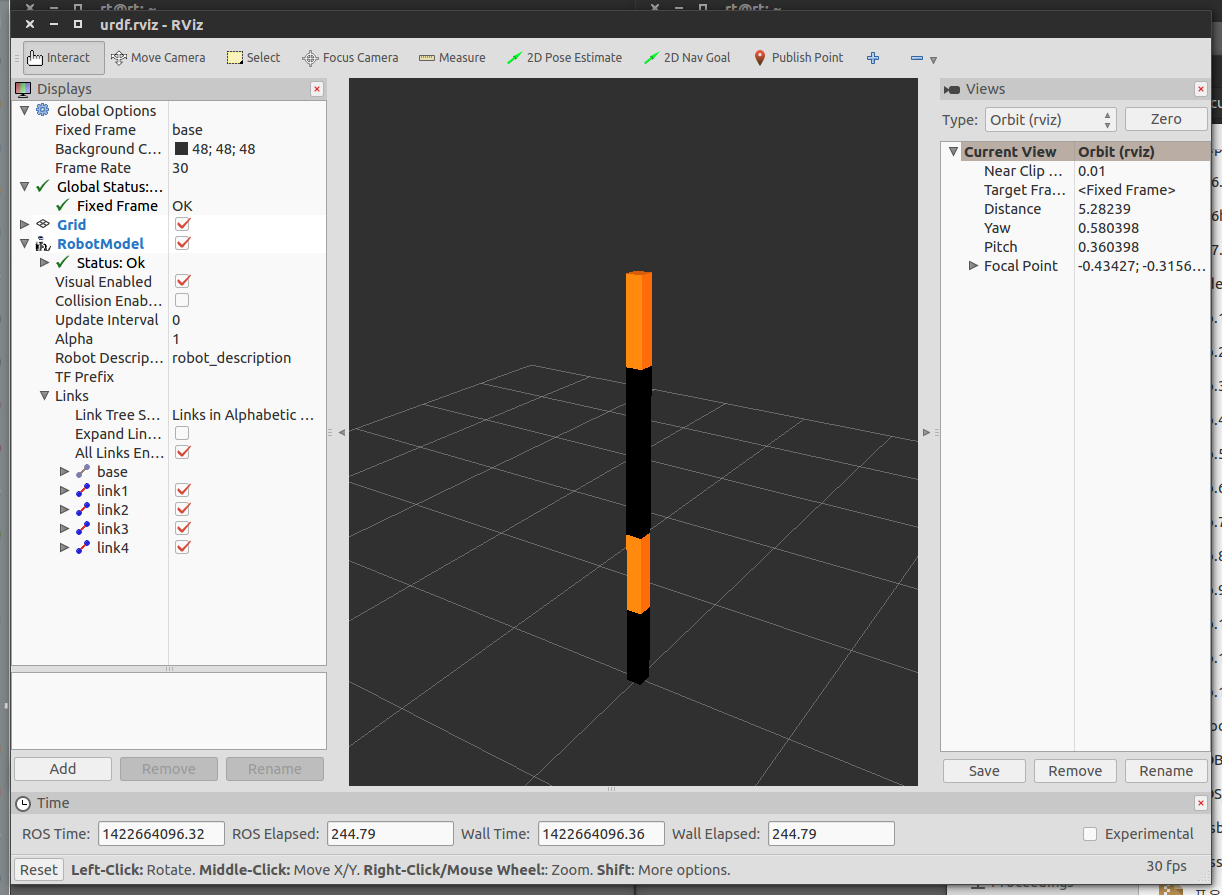
\includegraphics[width=10cm]{pictures/chapter11/pic_11_08.png}
  \caption{RVizによる関節とリンクの表示}
\end{figure}

\begin{figure}[htp]
  \centering
  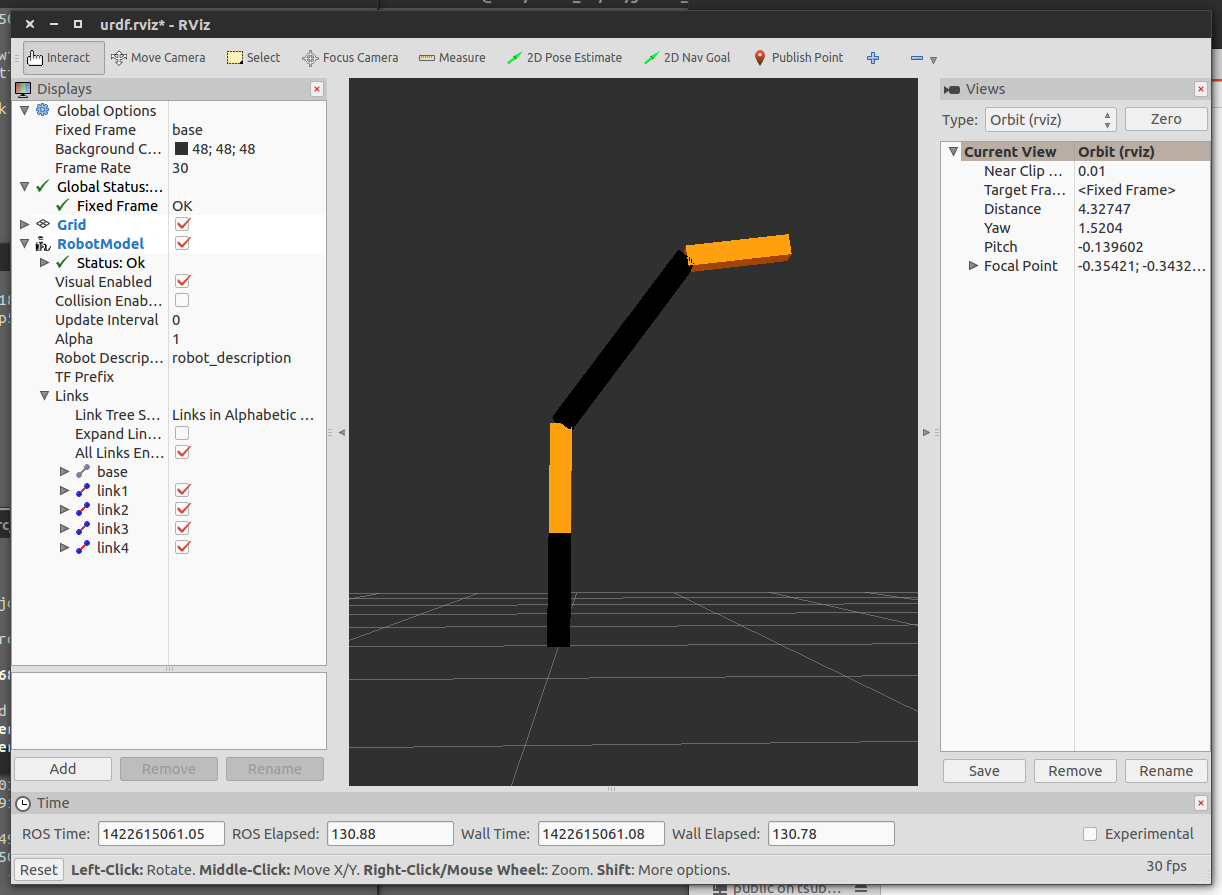
\includegraphics[width=10cm]{pictures/chapter11/pic_11_09.png}
  \caption{仮想ロボットの動作}
\end{figure}

%-------------------------------------------------------------------------------
\subsection{タートルボットアームのモデリング}

ここまで、3関節ロボットアームを例にURDFを作成する方法を説明してきた。この項では、より実際に近い例として、図11-10に示す4関節と開閉型グリッパーをもつロボットアームのモデリングを説明する。このロボットアームは、タートルボットアーム(turtlebot arm)注3という名前で販売されており、主にロボットアームの学習に用いられる。
タートルボットアームのベースは、タートルボットのフレームであり、関節アクチュエータにはRobotis社のDynamixel AX-12Aを使用している。エンドエフェクタの開閉型グリッパーなど、このアームで使用されている部品の3次元CADファイルは、「http://www.thingiverse.com/thing:5192」で公開されている。関連するハードウェアなどの説明は、http://wiki.ros.org/turtlebot\_armを参照してほしい。

\begin{figure}[htp]
  \centering
  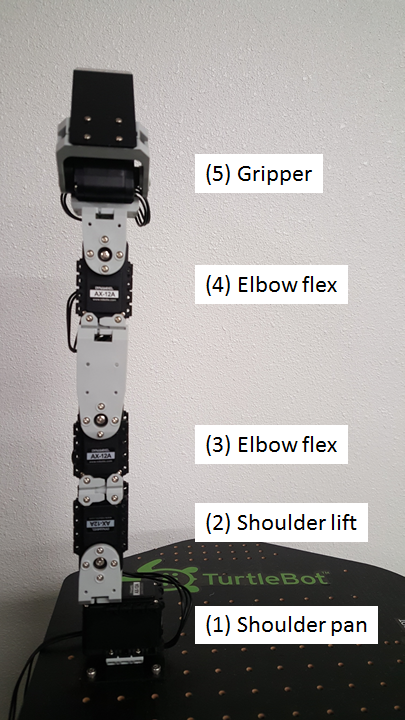
\includegraphics[width=10cm]{pictures/chapter11/pic_11_10.png}
  \caption{4関節+開閉型グリッパーを有するタートルボットアーム}
\end{figure}

本項で使用するパッケージは、URDF関連パッケージ、MoveIt、運動制御関連パッケージなどである。それぞれ、以下のようにインストールしておく。

\begin{lstlisting}[language=ROS]
$ sudo apt-get install liburdfdom-tools %*(11.4.1項でインストールしていない場合)*)
$ sudo apt-get install ros-indigo-moveit*
$ sudo apt-get install ros-indigo-arbotix*
$ sudo apt-get install ros-indigo-ros-control
$ sudo apt-get install ros-indigo-ros-controllers
$ sudo apt-get install ros-indigo-joint-state-controller
$ sudo apt-get install ros-indigo-effort-controllers
$ sudo apt-get install ros-indigo-position-controllers
$ sudo apt-get install ros-indigo-joint-trajectory-controller
\end{lstlisting}

その後、タートルボットアームの関連プログラム注4をダウンロードする。

\begin{lstlisting}[language=ROS]
$ cd ~/catkin_ws/src
$ git clone https://github.com/turtlebot/turtlebot_arm.git
\end{lstlisting}

以下のように、ダウンロードしたプログラムには、様々なパッケージが含まれている。

\begin{lstlisting}[language=ROS]
$ cd ~/catkin_ws/src/turtlebot_arm
$ ls
turtlebot_arm     %* → タートルボットアームのメタパッケージ*)
turtlebot_arm_block_manipulation     %* → ブロックを掴むpick\_and\_placeパッケージ*)
turtlebot_arm_bringup     %* → タートルボットアームの駆動パッケージ*)
turtlebot_arm_description     %* → タートルボットアームのモデルパッケージ*)
turtlebot_arm_ikfast_plugin        %* → ikfastベース逆運動学パッケージ*)
turtlebot_arm_kinect_calibration     %* → kinectのキャリブレーションパッケージ*)
turtlebot_arm_moveit_config     %* → moveit設定パッケージ*)
turtlebot_arm_moveit_demos     %* → moveitデモパッケージ*)
\end{lstlisting}

全てダウンロードしたら、ビルドする。

\begin{lstlisting}[language=ROS]
$ cd ~/catkin_ws
$ catkin_make
\end{lstlisting}

turtlebot\_arm\_descriptionに記述されたタートルボットアームのモデルを、11.4.1項で学んだcheck\_urdfやurdf\_to\_graphiz、RVizなどを用いて調べてみよう。タートルボットアームのモデルは、turtlebot\_arm\_descriptionパッケージのurdfフォルダにあるarm.urdfである。ターミナルウィンドウで確認する場合はcheck\_urdfを、グラフで確認したい場合はurdf\_to\_graphizを利用して、各関節とリンクとの関係について調べてみよう。

\begin{lstlisting}[language=ROS]
$ roscd turtlebot_arm_description
$ cd urdf
$ check_urdf arm.urdf
$ urdf_to_graphiz arm.urdf
\end{lstlisting}

urdf\_to\_graphizを利用した場合、turtlebot\_arm.pdfという名前のファイルが作成される。これを見ると、タートルボットアームは25個のリンクと24個の関節で表現されていることが分かる。ただし24個の関節のうち、18個は複数の部品(リンク)を固定するための固定関節である。

arm.urdfは、関節1(arm\_shoulder\_pan\_joint)、関節2(arm\_shoulder\_lift\_joint)、関節3(a\\rm\_elbow\_flex\_joint)、関節4(arm\_wrist\_flsx\_joint)、関節5(gripper\_link\_joint)、およびエンドエフェクタの開閉軸(gripper\_joint)をもつロボットアームである。ただし、関節5は、ikfast\_pluginを利用して逆運動学を解くために追加された受動関節(自らは駆動しない関節)であり、実際には存在しない。このため制御できる関節は、関節1~4の4関節とエンドエフェクタの1関節である。関節1〜5とエンドエフェクタの関節の種類はrevolute(回転関節)であり、残りの18個の関節はfixed(固定関節)である。
さらに、タートルボットアームのモデルをRVizで表示すると、図11-11に示すように、各関節(アクチュエータ、黒)とリンク(フレーム、白)が確認できる。先に述べた通りリンクは全部で25個あるが、大部分は固定関節で相互に結合されており、関節間は実質的に1つのリンクからなる。
次に、Joint State PublisherのGUIツールで各関節を動かしてみよう。次のようにtest.launchファイルを実行し、RVizの画面で「Fixed Frame」に「base\_link」を選択し、左下の<Add>ボタンを押して「RobotModel」を追加する。その後、joint\_state\_publisherノードのGUI画面で各関節のパラメータを変更すると、RViz上の仮想ロボットが動作する。ただし、gripper\_link\_jointは受動関節であり、関節のパラメータを変更しても何も動作しない。

\begin{lstlisting}[language=ROS]
$ roslaunch turtlebot_arm_description test.launch
$ rosrun rviz rviz
\end{lstlisting}

\begin{figure}[htp]
  \centering
  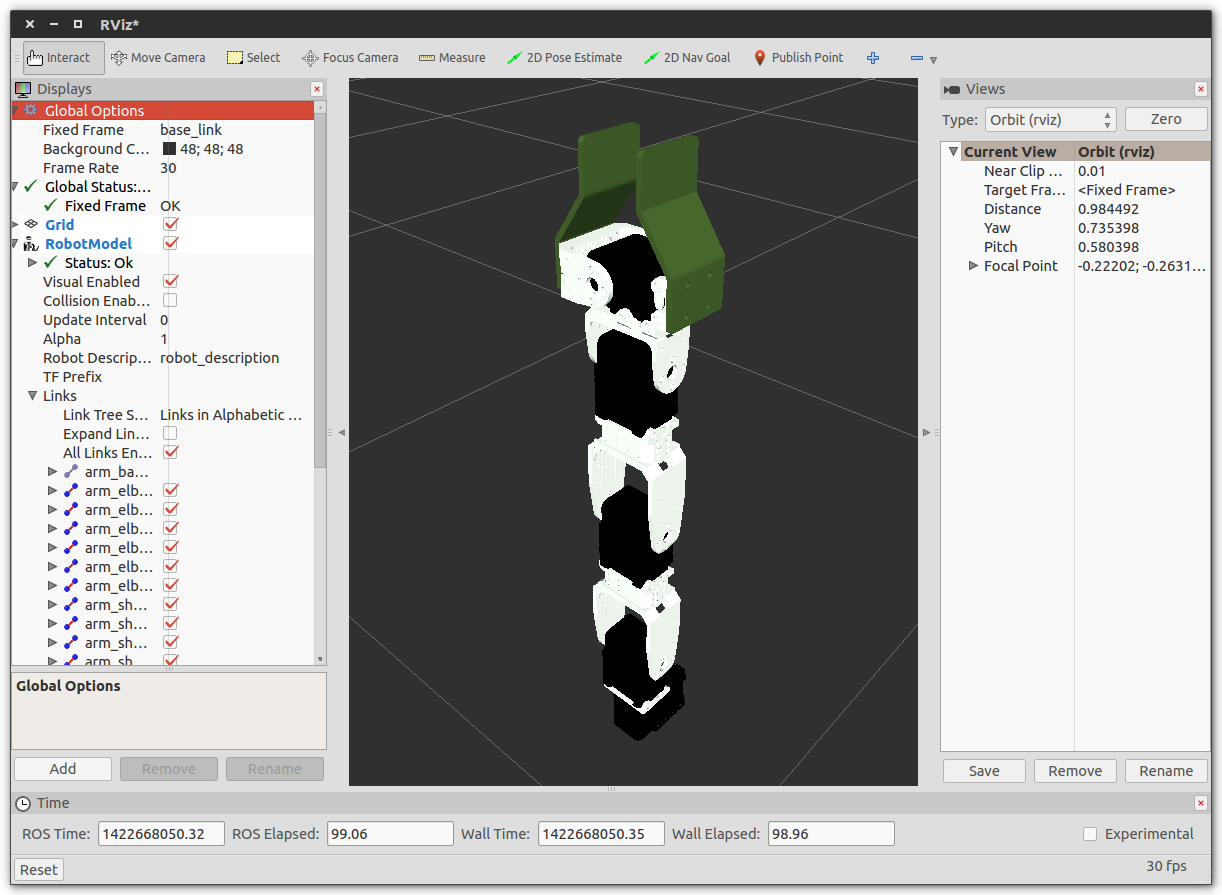
\includegraphics[width=12cm]{pictures/chapter11/pic_11_11.png}
  \caption{RVizによる関節、リンク、グリッパーの表示}
\end{figure}

\begin{exercise}[Xacroファイル]
turtlebot\_arm\_description/urdfのモデリングファイルを見ると、「*.xacro」というファイルがある。これは、XMLマクロ言語で記述されたXML Macrosファイルである。URDF形式では、要素一つ一つは簡潔に作られているが、関節やリンク数が多くなると、類似した要素が繰り返され、ソースコードが読みにくくなる。また、複数個所で使われている変数名を変更する際、何度も修正を繰り返す必要がある。しかしxacroを使えば、URDFの属性を再利用することで、読みやすい記述が実現できる。xacroの使用方法はhttp://wiki.ros.org/xacroを参照してほしい。なお、xacroで作成されたモデルファイルは、次のようにxacroパッケージを利用してurdfに自動的に変換できる。

\begin{lstlisting}[language=ROS]
$ rosrun xacro xacro.py arm.urdf.xacro > arm.urdf
\end{lstlisting}
\end{exercise}

%-------------------------------------------------------------------------------
\section{MoveItを用いたロボットアームの動作計画}\index{MoveItを用いたロボットアームの動作計画}

MoveItは、動作計画、3次元知覚、運動学計算、制御などを提供するパッケージである。特に、ロボットで頻繁に取り扱うロボットアームの順運動学計算と逆運動学計算が可能であり、物体把持やピック&プレイス作業などが簡単に実行できる。
MoveItで使用できるロボットアームは、前節で紹介したタートルボットアームのほかに、65種以上もある注5。ここでは、MoveItを用いて、タートルボットアームの動作計画を行ってみる。

%-------------------------------------------------------------------------------
\subsection{MoveItの処理手順}

本稿では、MoveItの内部で行われる処理手順の概要を説明する。MoveItのシステムアーキテクチャを図11-12に示す。MoveItは動作計画を行うノードなど、個々のノードと外部とのインターフェースの役割を担うmove\_groupノード注6を中心に構成されている。MoveItを起動すると、move\_groupのノードはROSパラメータサーバよりロボットモデルと環境変数をURDF、SRDF、Config形式で受けとる。また、move\_groupノードはロボットの各関節値の情報であるJoint Stateトピックと、各関節とリンクの相対位置関係を記述したtfトピックを受け取り、ロボットの現在の姿勢を計算する。さらに、ロボットが把持する物体として、RViz上に仮想的に存在する物体、もしくはKinectやXtionなどのデプスカメラから取得した点群(Point Cloud)形式の物体の情報が与えられる。
ユーザーは、move\_group\_interface(C ++)、moveit\_commander(Python)、RViz PluginのGUI画面などのユーザインターフェースを介し、move\_groupノードに接続して作業コマンドを送信する。move\_groupノードは、ユーザーから作業コマンドを受信すると、MoveItの主要コンポーネントの一つであるOMPL(Open Motion Planning Library、動作計画ライブラリ)、ロボットの姿勢、センサ情報、把持物体や障害物の幾何情報(Planning Scene)、順運動学・逆運動学プラグイン、衝突チェック機能などを使用して、必要な動作を自動生成する。最後に、Robot Controllersノードに、生成された作業動作を実現する各関節の関節軌道(Joint Trajectory)を渡すことで、ロボットが計画通りに動作する。

\begin{figure}[htp]
  \centering
  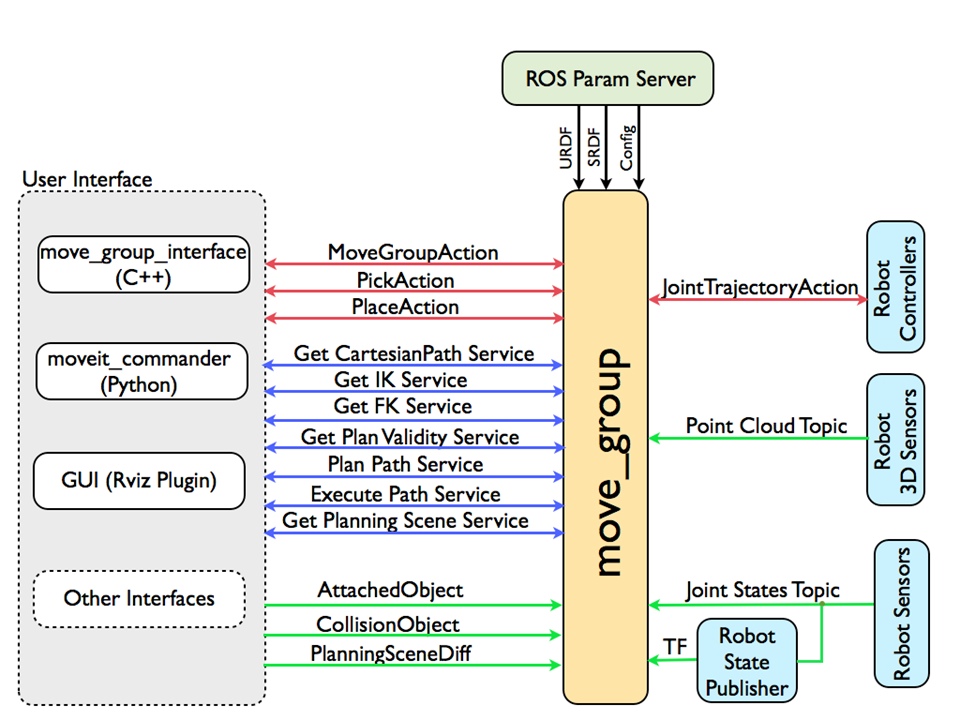
\includegraphics[width=12cm]{pictures/chapter11/pic_11_12.png}
  \caption{MoveItのシステムアーキテクチャ(http://moveit.ros.org/documentation/concepts/)}
\end{figure}


\begin{exercise}[SRDF(Semantic Robot Description Format)とは]
SRDF注7は、MoveItでの動作計画で用いられるロボットの記述方式である。URDF(Universal Robot Description Format)の文法を一部採用しているが、URDFを拡張または置き換えるものではなく、意味(Semantic)情報を記述するための方式である。MoveItの「MoveIt Setup Assistant」を使用すると、作成しておいたURDFファイルを参照して、SRDFファイルを生成することができる。ちなみにGazeboシミュレータでは、シミュレーションに必要な仮想空間、光、物理的な力、センサ、衝突、視覚化、ロボットや物体などのモデルを記述できるSDF(Simulation Description Format、http://sdformat.org/)フォーマットを使用している。SRDF, URDF, SDFの違いは、次のWikiに詳しい。

http://wiki.ros.org/ROS/Patterns/RobotModelling
\end{exercise}

%-------------------------------------------------------------------------------
\subsection{MoveIt Setup Assistantを用いた設定ファイルの作成}

MoveItを使用するには、あらかじめ作成しておいたURDF形式のロボットモデルをSRDF形式(コラム「SRDF(Semantic Robot Description Format)とは」参照)に変換し、MoveItに必要な設定を追加すればよい。しかし、これは簡単な作業ではない。設定作業を支援するGUIツールとして、MoveItではMoveIt Setup Assistant注8が提供されている。以下では、このツールの使用法について説明する。
まず、次のようにmoveit\_setup\_assistant.launchを実行する。

\begin{lstlisting}[language=ROS]
$ roslaunch moveit_setup_assistant setup_assistant.launch
\end{lstlisting}

\subsubsection{設定ファイルの読み込み}

MoveIt Setup Assistantを実行すると、図11-13のようなGUI画面が現れる。ここでは、[Choose mode]が2つあり、左ボタンをクリックすると、ユーザーが指定したURDFから設定を開始する。右ボタンをクリックした場合は、既存の設定ファイルから設定を読み込み、作業を開始する。新しいロボットであれば左ボタンをクリックするが、ここではタートルボットアームについて説明するため、右ボタンを押す。

\begin{figure}[htp]
  \centering
  
\includegraphics[width=12cm]{pictures/chapter11/pic_11_13.png}
  \caption{MoveIt Setup Assistantの初期画面}
\end{figure}

[Choose mode]で右ボタンをクリックすると、図11-14のように、既存のMoveIt設定パッケージのアドレスを入力する部分が現れる。<Browse>ボタンを押してturtlebot\_arm\_moveit\_configパッケージが保存された場所を選択する。 turtlebot\_arm\_moveit\_configパッケージは、11.4.2項に従ってダウンロードしていれば、次の場所にある。

/home/[ユーザー名]/catkin\_ws/src/turtlebot\_arm/turtlebot\_arm\_moveit\_config

turtlebot\_arm\_moveit\_configフォルダを選択して、<Load Files>ボタンをクリックし、既存の設定ファイルを開く。

\begin{figure}[htp]
  \centering
  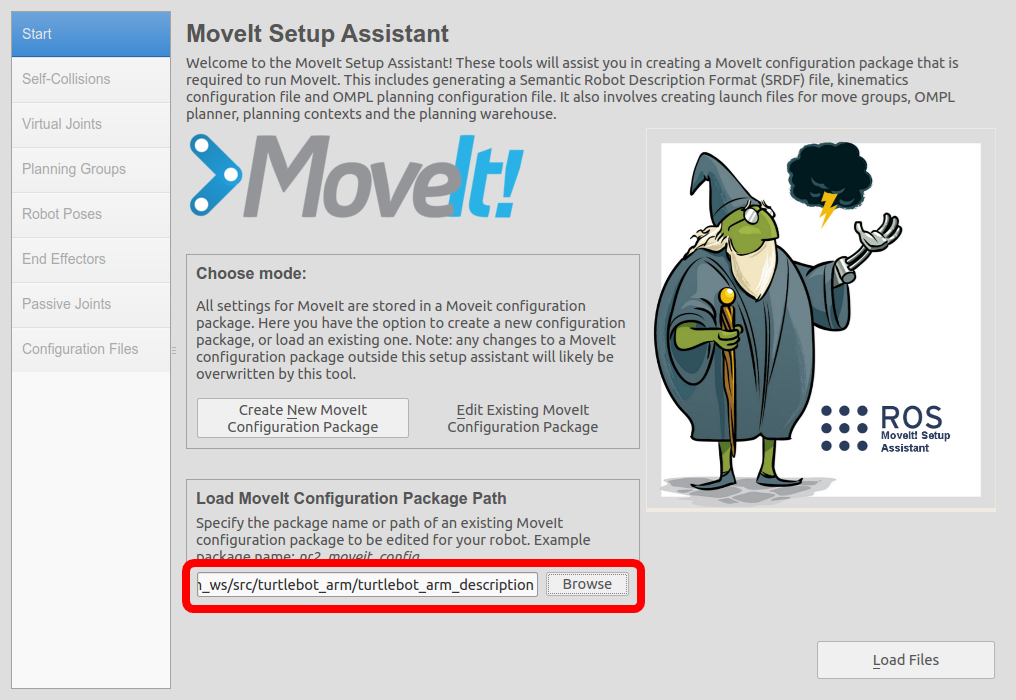
\includegraphics[width=12cm]{pictures/chapter11/pic_11_14.png}
  \caption{MoveIt Setup Assistantでの設定ファイルの読み込み}
\end{figure}

読み込みが終わると、図11-15のように、画面の右側にロボットが表示される。

\begin{figure}[htp]
  \centering
  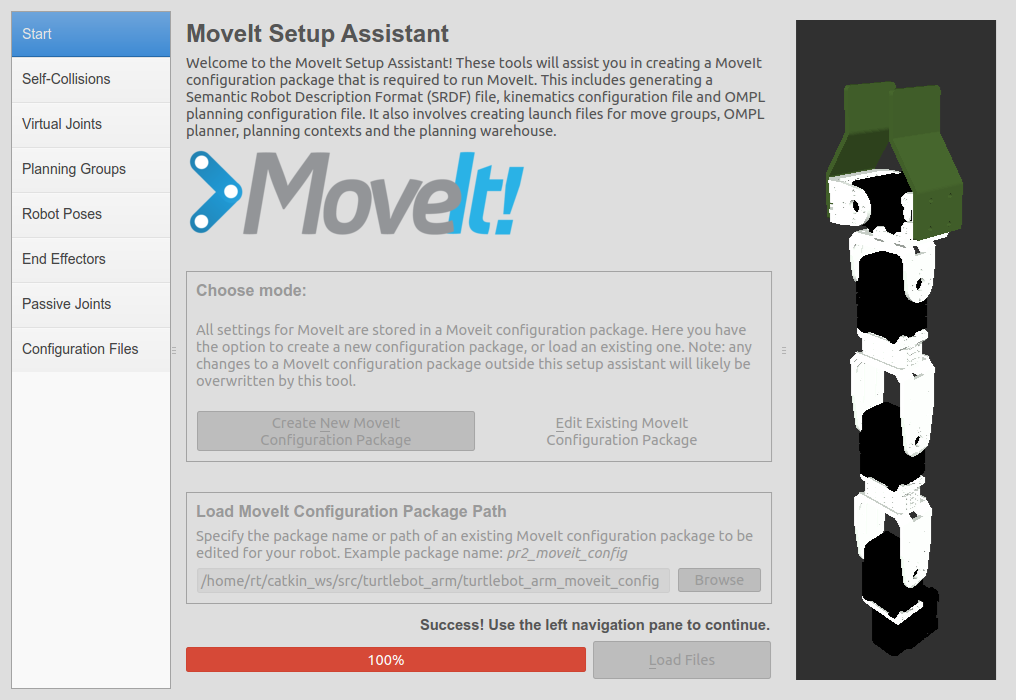
\includegraphics[width=12cm]{pictures/chapter11/pic_11_15.png}
  \caption{MoveIt Setup Assistant でのロボットの表示}
\end{figure}

\subsubsection{自己干渉(Self-Collisions)}

自己干渉オプションは、リンク間の幾何学的な接触に対して、常に接触している部分、絶対接触することがない部分を予め設定し、MoveItの干渉チェックで判定しないように設定するオプションである。今回読み込んだモデルでは、図11-16のように自己干渉オプションが既に設定されている。もし、新たに作成したロボットであれば、<Regeneratre Default Collision Matrix>ボタンをクリックすれば、己干渉オプションが設定される。

\begin{figure}[htp]
  \centering
  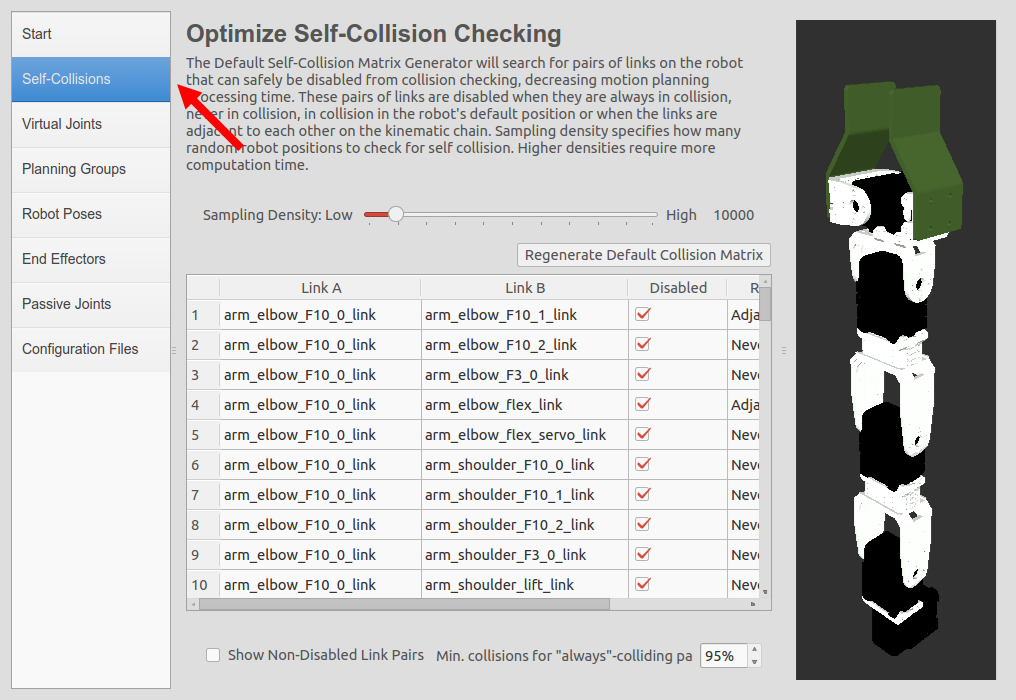
\includegraphics[width=12cm]{pictures/chapter11/pic_11_16.png}
  \caption{自己干渉の設定}
\end{figure}

\subsubsection{仮想関節(Virtual Joints)}

フレーム間に仮想的な関節を設定するオプションである。(図11-17)MoveItで床面を移動する移動ロボットを用いる場合は、床上をスライドできる平面拘束関節(planar)を設定する。本項では、床面に固定されたロボットアームを用いるので、設定する必要はない。

\begin{figure}[htp]
  \centering
  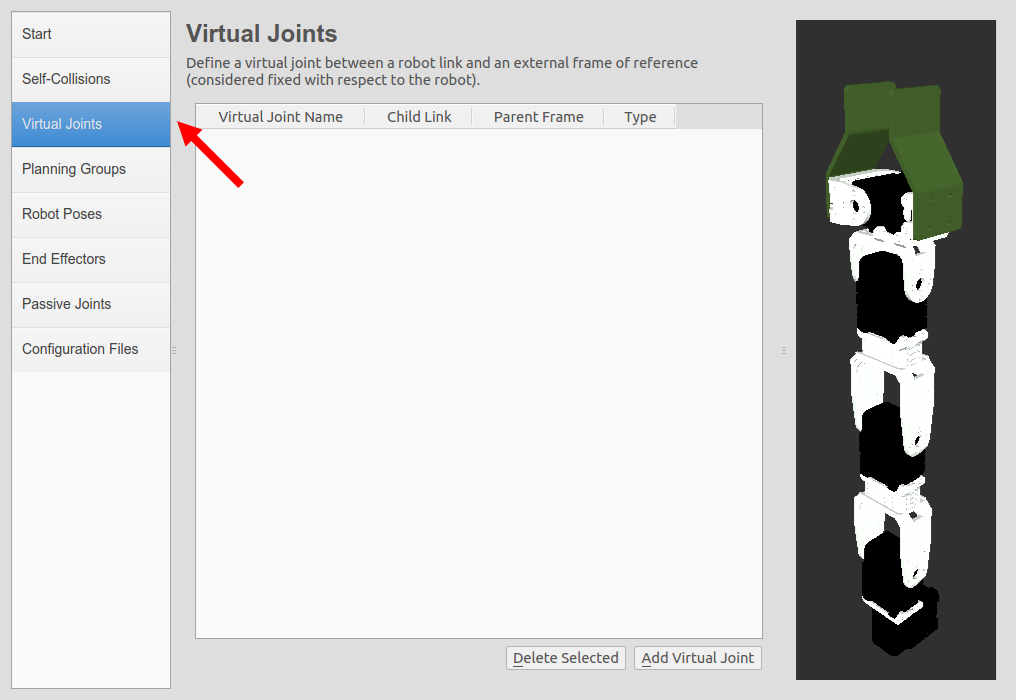
\includegraphics[width=12cm]{pictures/chapter11/pic_11_17.png}
  \caption{仮想関節の設定画面}
\end{figure}

\subsubsection{プランニンググループ(Planning Groups)}

ロボットアームの要素をグループに分け、グループごとの作業計画を可能にする。タートルボットアームの場合、図11-18に示すように、ロボットアーム本体のarmグループとエンドエフェクタのgripperグループの2つに分かれる。まず、gripperについて説明する。

\begin{figure}[htp]
  \centering
  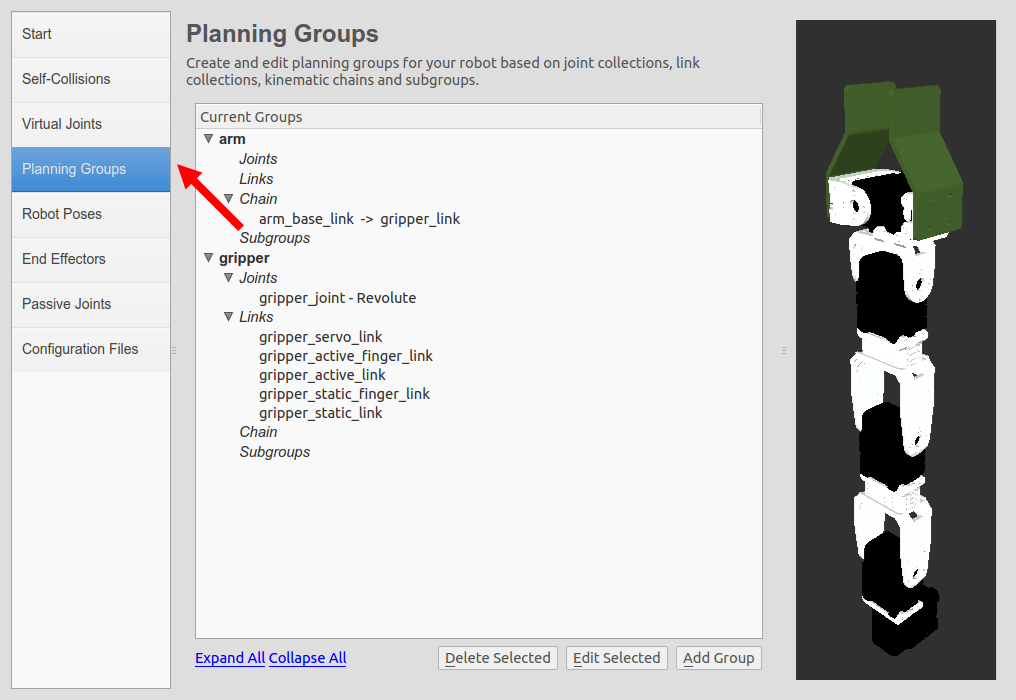
\includegraphics[width=12cm]{pictures/chapter11/pic_11_18.png}
  \caption{プランニンググループ}
\end{figure}

中央画面の太字のgripper を選択して、Edit Selectedボタンを押すと、gripperグループの設定が確認できる。ここでは、図11-19のように名前、運動学ソルバ(Solver)のプラグイン名、運動学計算の分解能、制限時間、試行回数などが設定されている。ここで、通常は運動学ソルバにはkdl\_kinematics\_plugin/KDLKine\\maticsPluginを、分解能、制限時間、試行回数は初期値をそのまま設定する。しかし、タートルボットアームのグリッパーは機構が単純で運動学ソルバを必要としないため設定しない。確認したら、Cancelを押して、元の画面に戻る。

\begin{figure}[htp]
  \centering
  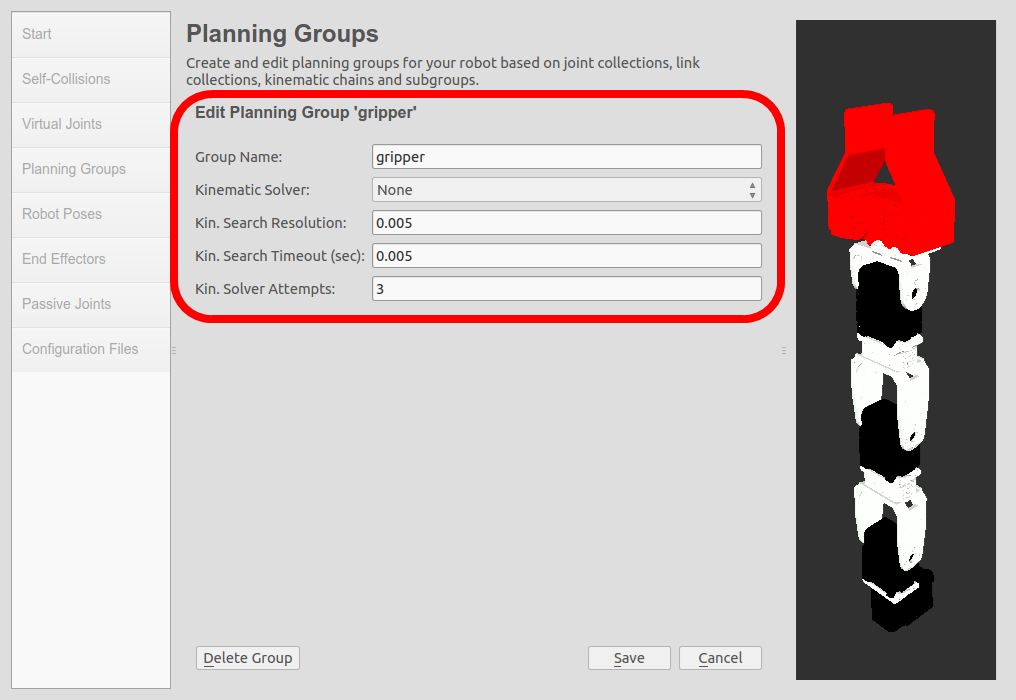
\includegraphics[width=12cm]{pictures/chapter11/pic_11_19.png}
  \caption{グリッパーグループの設定}
\end{figure}

図11-18のように、画面中央のCurrent Groupsの欄には、プランニンググループごとに [Joints]、[Links]、[Chain]、[Subgroups]の項目が表示されている。[Joints]を選択してEdit Selectedボタンを押すと、図11-20のようにグループに登録する関節名の選択画面が現れる。登録する関節を選択して入力するが、既に設定済みであり、キャンセルを押して元の画面に戻る。[Links]は、図11-21のようにグリッパーを構成するすべてのリンクを設定しておく。[Chain]は、ベースから末端のリンクまでが運動学チェーン(運動学を計算するリンクと関節の並び)であることを設定する。[Subgroups]は、グループの下にサブグループが存在する場合に使用され、通常は使用しない。

\begin{figure}[htp]
  \centering
  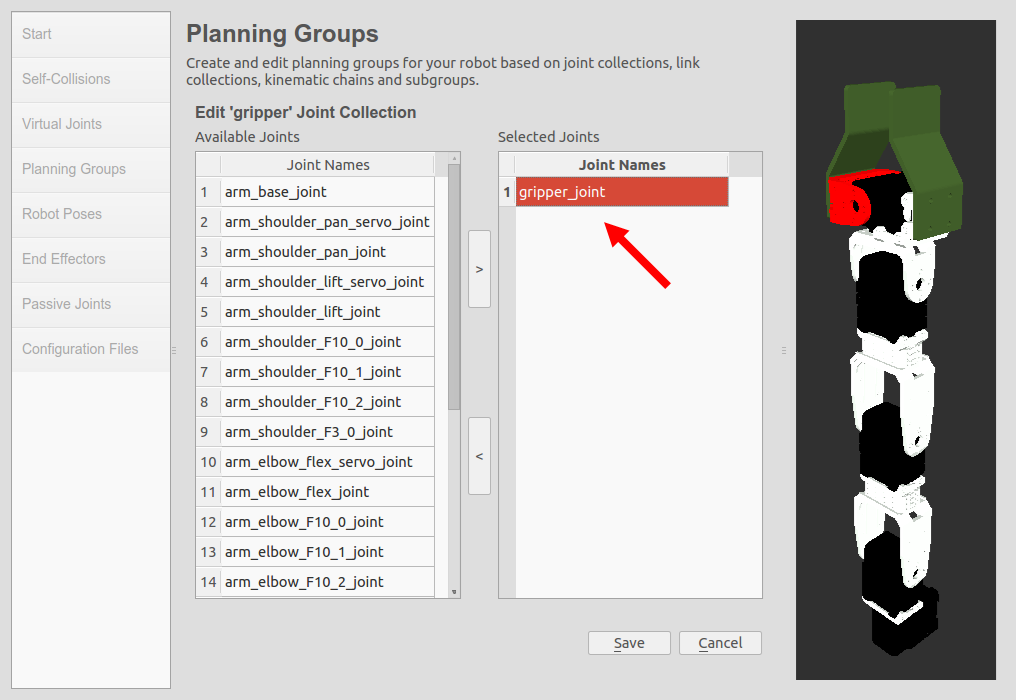
\includegraphics[width=12cm]{pictures/chapter11/pic_11_20.png}
  \caption{プランニンググループにおけるJoints項目の設定}
\end{figure}

\begin{figure}[htp]
  \centering
  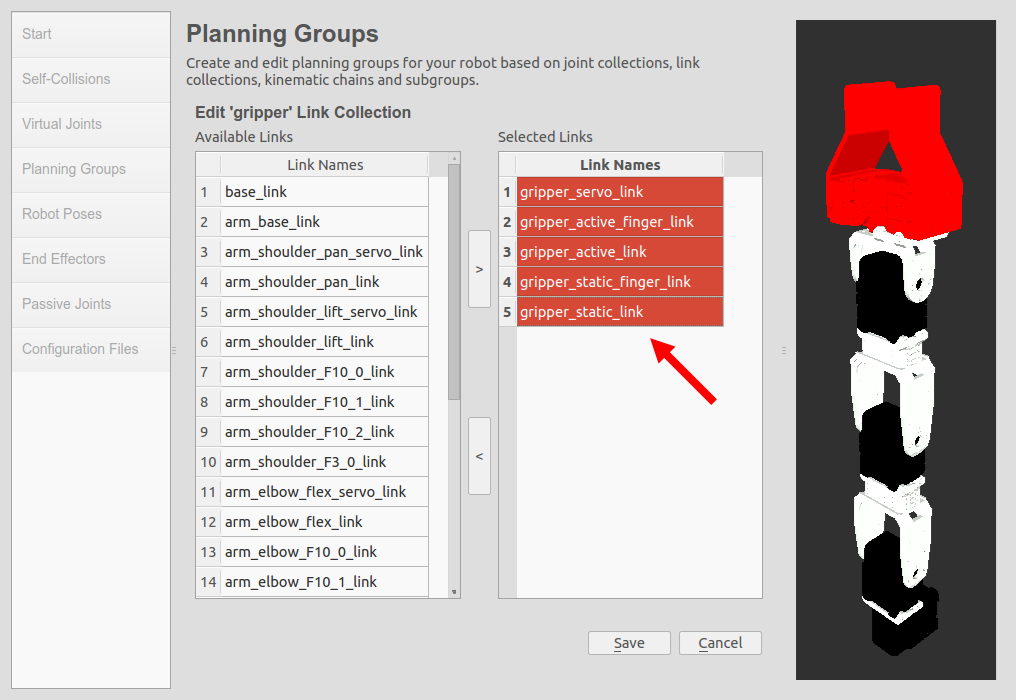
\includegraphics[width=12cm]{pictures/chapter11/pic_11_21.png}
  \caption{プランニンググループにおけるLinks項目の設定}
\end{figure}

次に、armグループについて説明する。armグループには、図11-18に示すように、[Joints]や[Links]の情報が設定されていない。一般的なロボットアームの場合、運動学ソルバとしてMoveItで提供される標準の6自由度アーム用KDLKinematicsPlugin注9を用いるには、図11-22、図11-23のように関節(arm\_sho\\ulder\_pan\_joint、arm\_shoulder\_lift\_joint、arm\_elbow\_flex\_joint、arm\_wrist\_flsx\_joint)\\やリンク(arm\_base\_linkからarm\_wrist\_F3\_0\_linkまで)の情報を入力して、図11-24のように設定しなければならない。しかし、 armグループのロボットアームは4自由度なので、6自由度アーム用KDLKinematicsPluginを用いることができない。そこで、4つのアクチュエータに1つの受動関節を追加した5関節モデルを作り、図11-25のように運動学ソルバにIKFASTKinematicsPlugin注10を設定した。この場合、図11-18に示すように、関節とリンク情報は設定する必要はなく、chain情報のみを記述する。

\begin{figure}[htp]
  \centering
  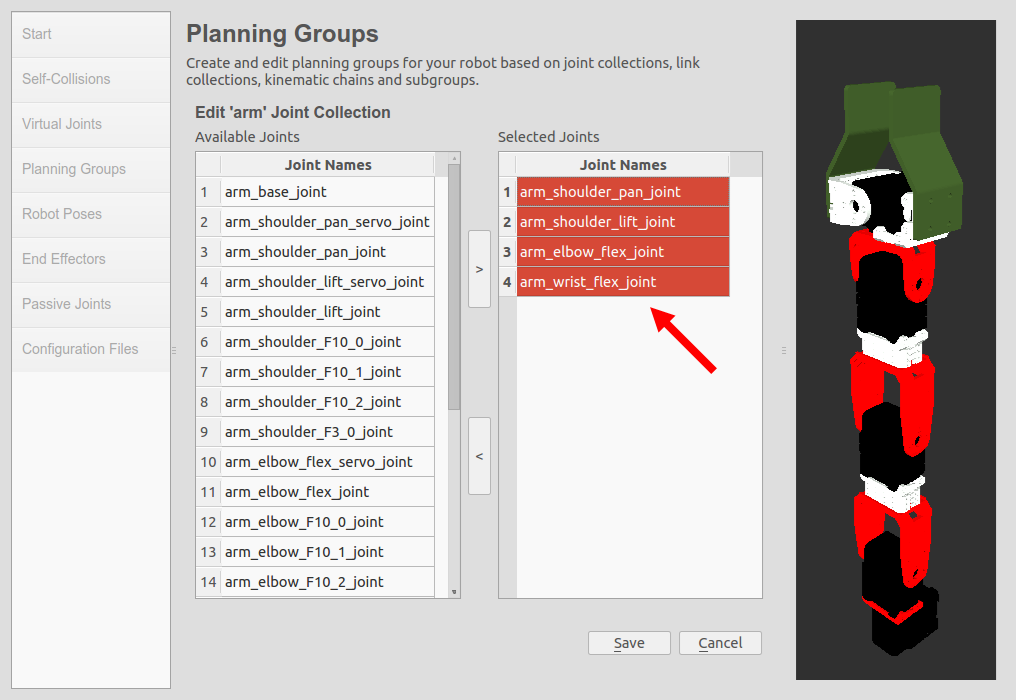
\includegraphics[width=12cm]{pictures/chapter11/pic_11_22.png}
  \caption{一般的なロボットアームでの関節情報の登録}
\end{figure}

\begin{figure}[htp]
  \centering
  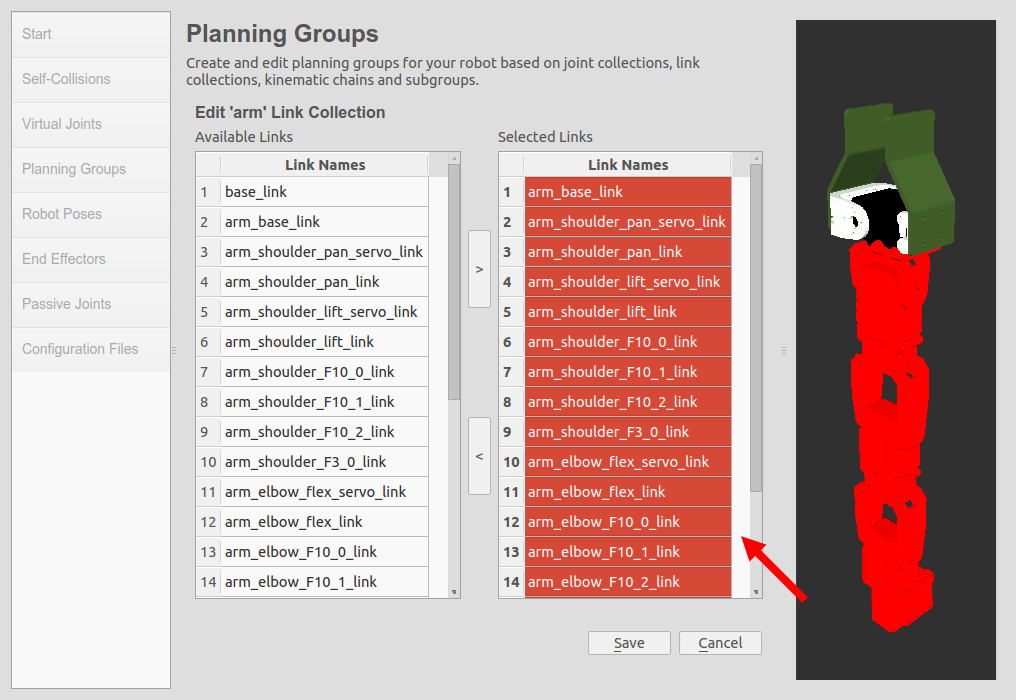
\includegraphics[width=12cm]{pictures/chapter11/pic_11_23.png}
  \caption{一般的なロボットアームでのリンク情報の登録}
\end{figure}

\begin{figure}[htp]
  \centering
  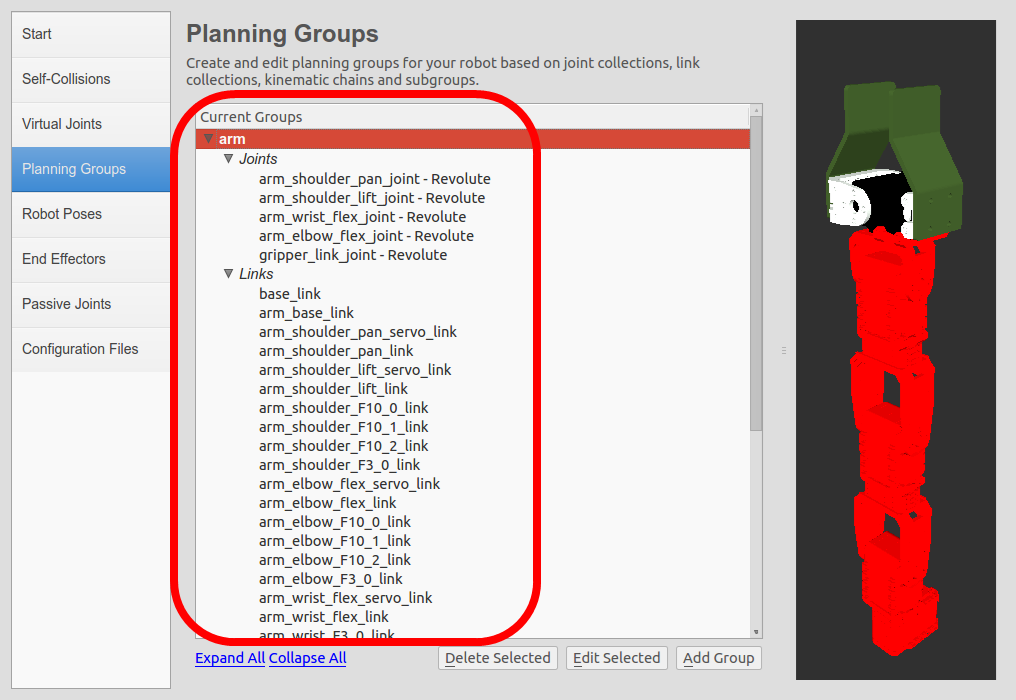
\includegraphics[width=12cm]{pictures/chapter11/pic_11_24.png}
  \caption{一般的なロボットアームに対する登録結果}
\end{figure}

\begin{figure}[htp]
  \centering
  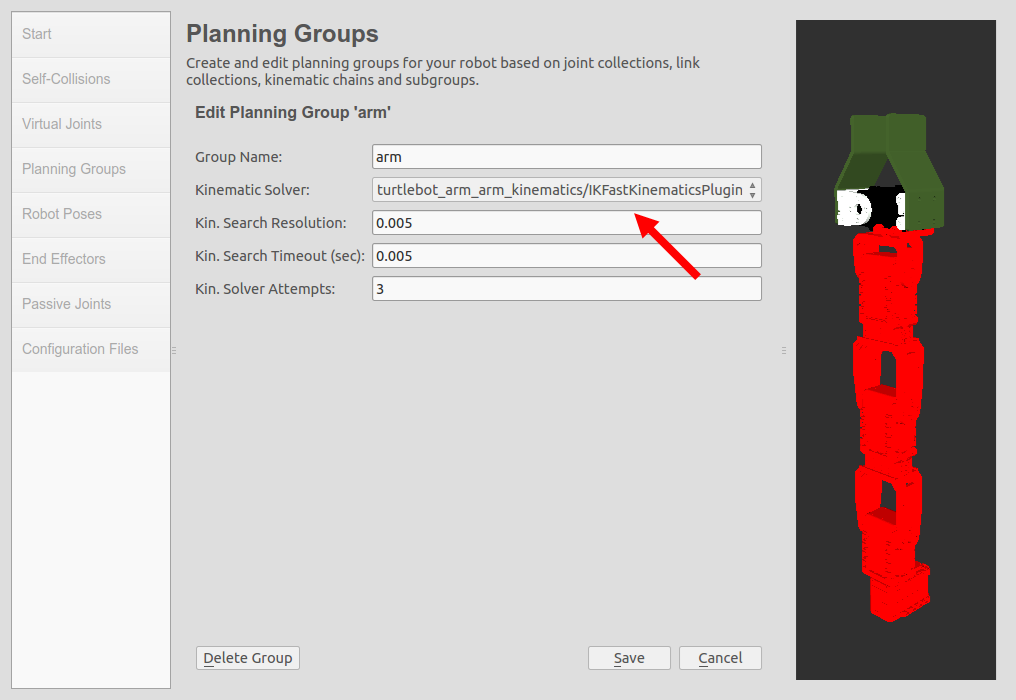
\includegraphics[width=12cm]{pictures/chapter11/pic_11_25.png}
  \caption{運動学ソルバにIKFASTKinematicsPluginを設定}
\end{figure}

\subsubsection{ロボットの姿勢(Robot Poses)}

MoveItでは、ロボットアームの複数の姿勢を事前に登録できる。例えば、図11-26のような最もコンパクトな姿勢や、図11-27のようなすべての関節が伸びた姿勢などである。新たな姿勢を登録するには、右下のAdd Poseボタンを押して、図11-28の画面で右側のスライダを動かして姿勢を調整する。目的の姿勢が決まったら、Pose Name欄に名前を入力して、Saveボタンを押す。

\begin{figure}[htp]
  \centering
  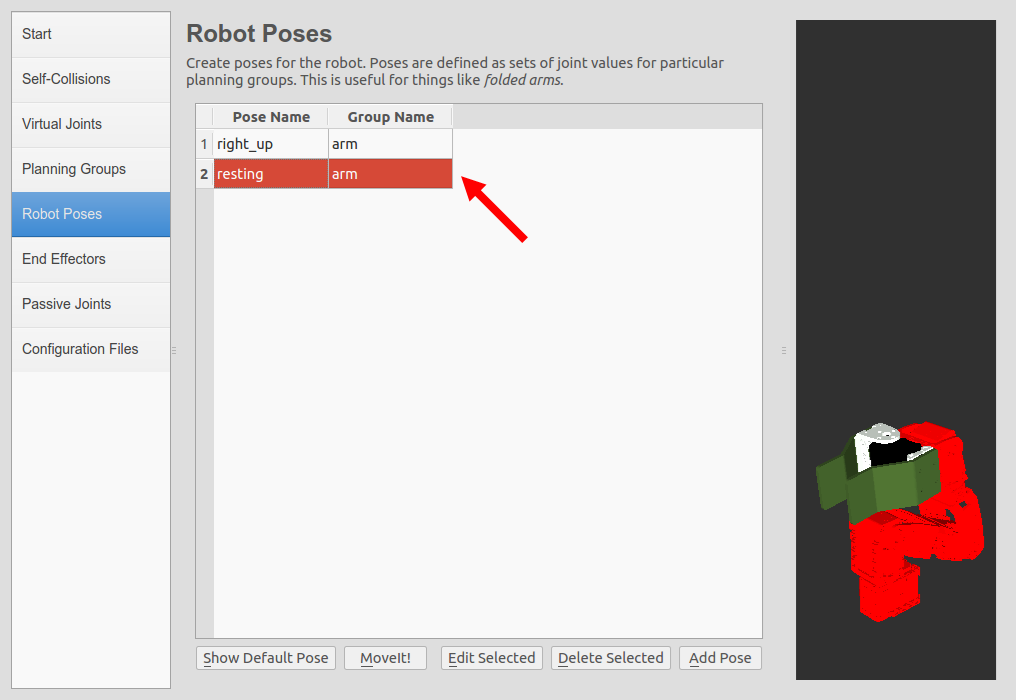
\includegraphics[width=12cm]{pictures/chapter11/pic_11_26.png}
  \caption{登録された姿勢の例(最もコンパクトな姿勢)}
\end{figure}
%図11-27 

\begin{figure}[htp]
  \centering
  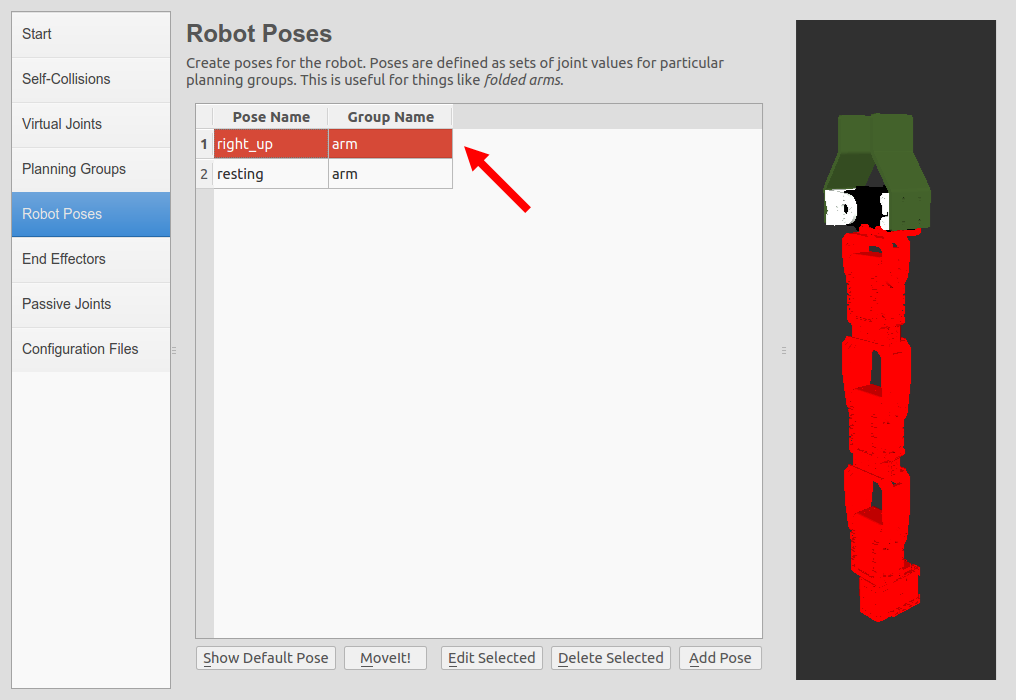
\includegraphics[width=12cm]{pictures/chapter11/pic_11_27.png}
  \caption{登録された姿勢の例(すべての関節が伸びた姿勢)}
\end{figure}
%図11-28 

\begin{figure}[htp]
  \centering
  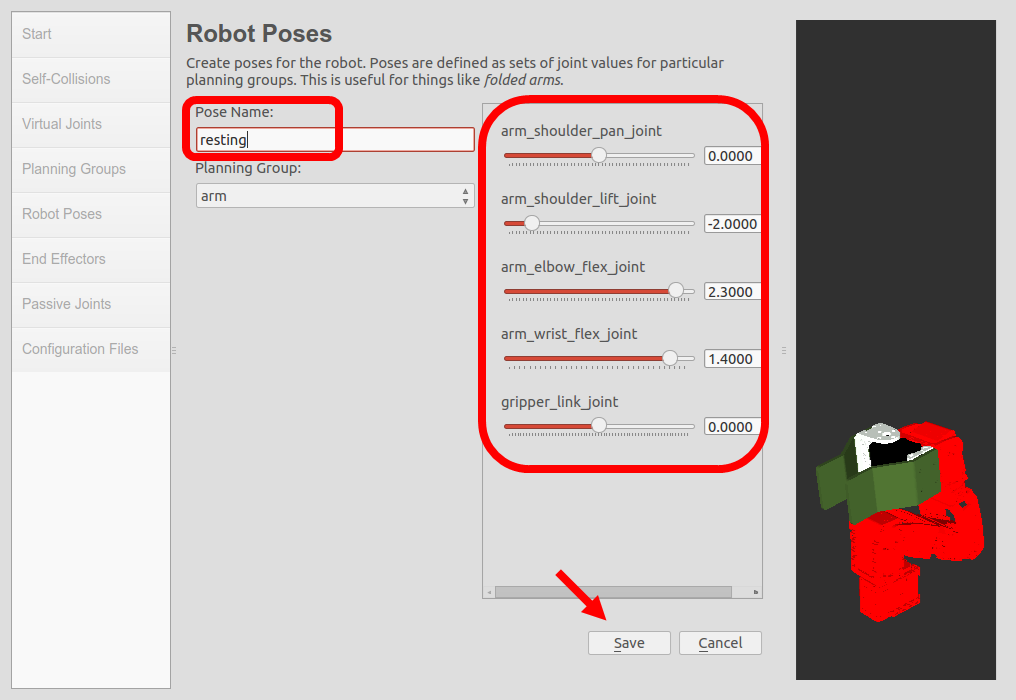
\includegraphics[width=12cm]{pictures/chapter11/pic_11_28.png}
  \caption{姿勢の登録方法}
\end{figure}

\subsubsection{エンドエフェクタ(End Effectors)}

エンドエフェクタの設定では、グリッパーや多指ハンドなどのエンドエフェクタの情報を設定する。図11-29のAdd End Effectorボタンを押すと、図11-30のようにグリッパーの名前、グループ名、親リンク、親グループの情報を入力する欄が現れる。既に設定されているgripperという名前のエンドエフェクタでは、グループ名はgripper、親リンクがgripper\_link、親グループの情報がarmとなっている。

\begin{figure}[htp]
  \centering
  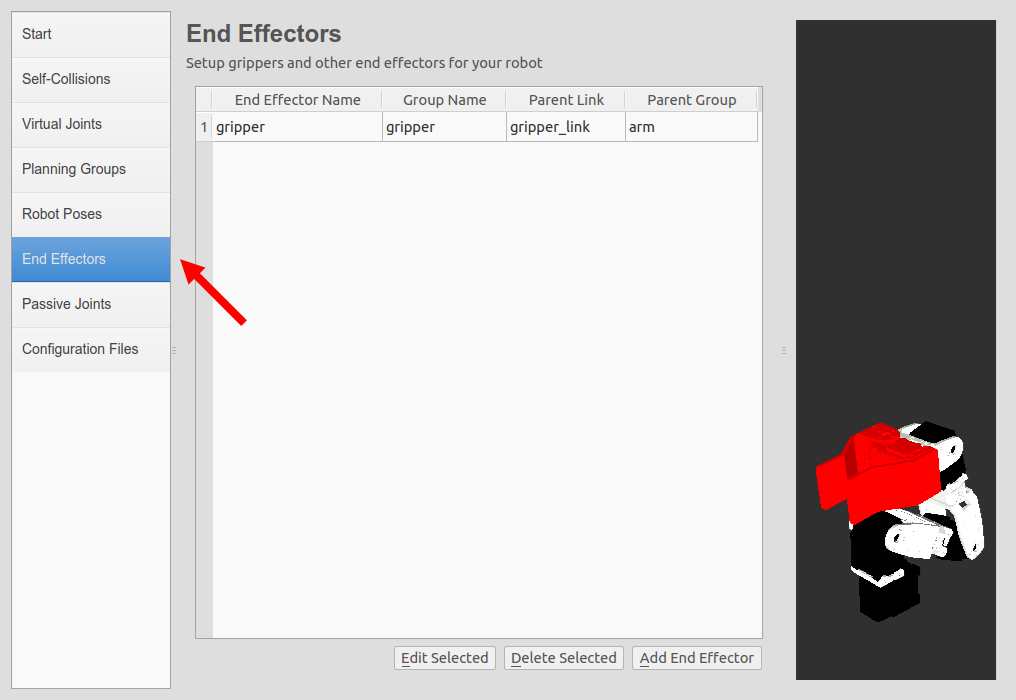
\includegraphics[width=12cm]{pictures/chapter11/pic_11_29.png}
  \caption{エンドエフェクタ(グリッパー)の設定}
\end{figure}

\begin{figure}[htp]
  \centering
  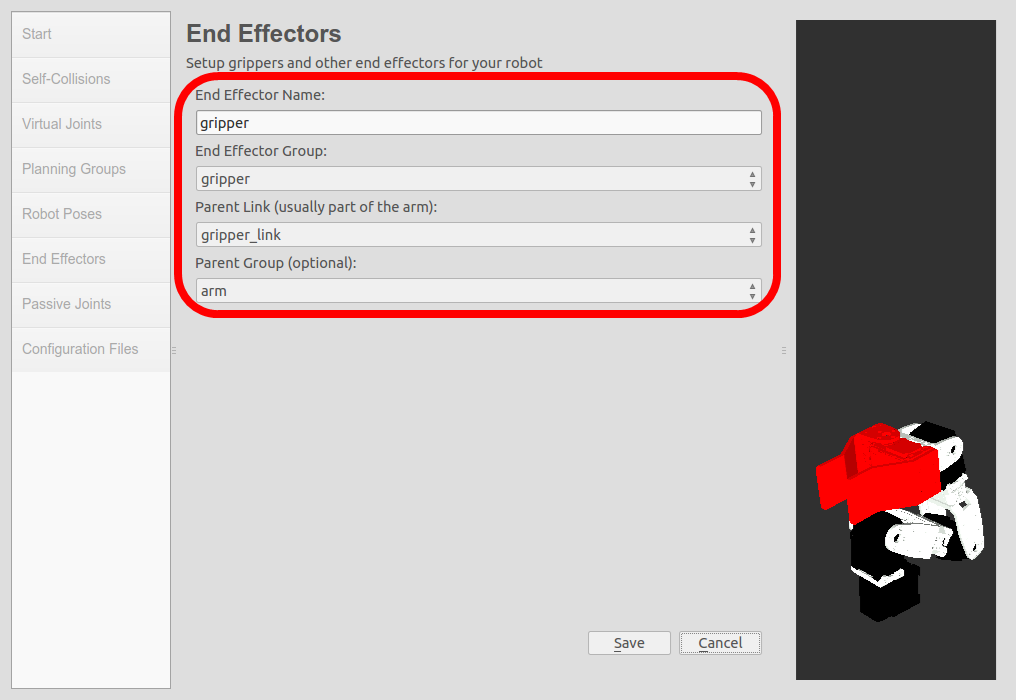
\includegraphics[width=12cm]{pictures/chapter11/pic_11_30.png}
  \caption{エンドエフェクタの情報入力}
\end{figure}

\subsubsection{受動関節(Passive Joints)}

モデルに受動関節がある場合には、ここで設定する。タートルボットアームでは、gripper\_link\_jointを受動関節として使用しているので、Active Joints欄の一覧からgripper\_link\_jointを選択して、Passive Joints欄に登録する。

\begin{figure}[htp]
  \centering
  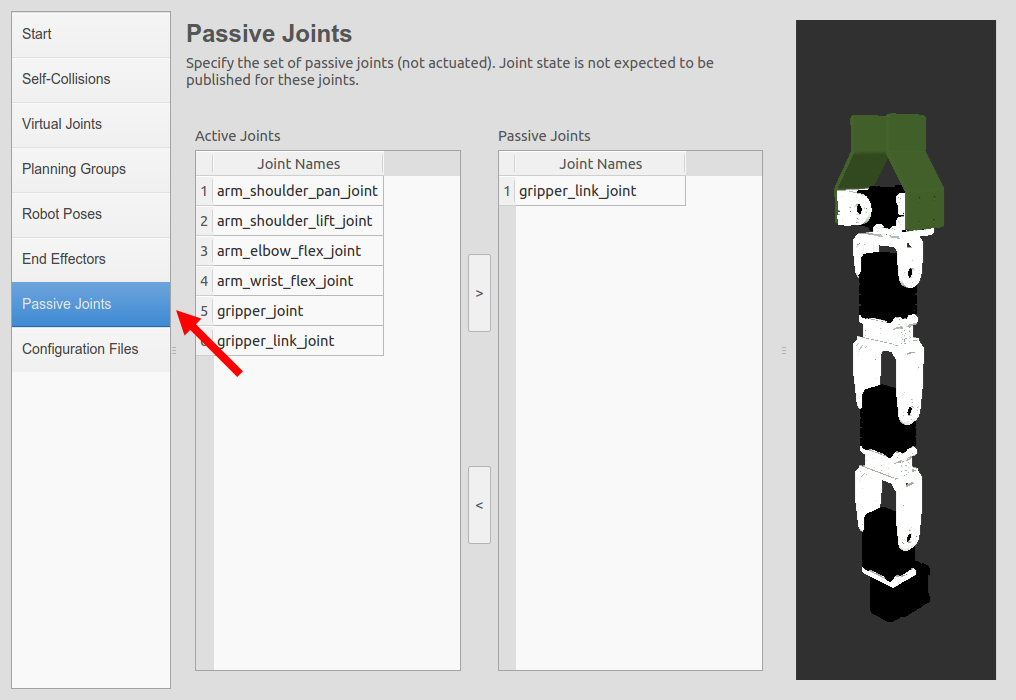
\includegraphics[width=12cm]{pictures/chapter11/pic_11_31.png}
  \caption{受動関節の設定}
\end{figure}

\subsubsection{設定ファイル(Configuration Files)}

最後に、図11-32のようにMoviItを使用するための設定ファイルを生成する。これらは、SRDF形式のアームのモデル、運動学計算で必要な関節とリンクの設定ファイル、launchファイルなど、25種以上の設定ファイルからなる。これらの設定ファイルの保存場所は任意に選べ、また必要な設定ファイルだけ選択して保存できる。ここでは全てのチェックボタンにチェックを入れ、右下の<Generate Package>をクリックすると、指定した保存場所に設定ファイルが生成される。その後、<Exit Setup Assitant>をクリックすると、セットアップが終了する。

\begin{figure}[htp]
  \centering
  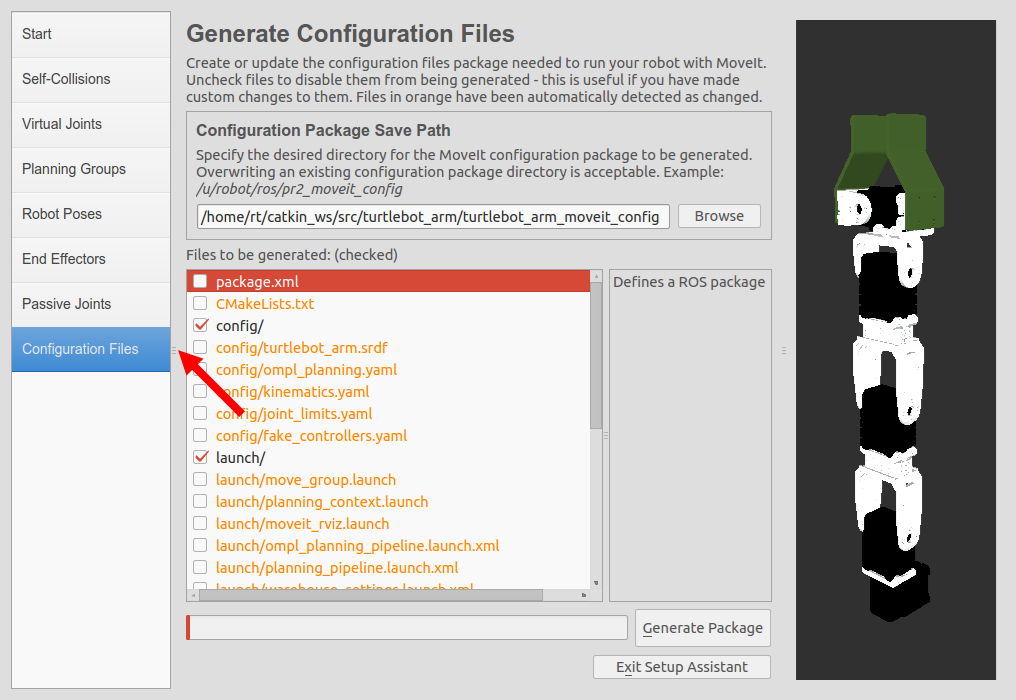
\includegraphics[width=12cm]{pictures/chapter11/pic_11_32.png}
  \caption{設定ファイルの生成}
\end{figure}

%-------------------------------------------------------------------------------
\subsection{MoveItを利用した逆運動学の動作テスト}

すべての設定が終わったら、次に、MoveItでタートルボットアームの動作テストをしよう。次の例のようにturtlebot\_arm\_moveit.launchを実行すると、RVizが起動する。

\begin{lstlisting}[language=ROS]
$ roslaunch turtlebot_arm_moveit_config turtlebot_arm_moveit.launch
\end{lstlisting}

図11-33に示すように、RVizの右側のウィンドウには、ロボットモデルと緑色のボールマーカ、ボールマーカの位置と姿勢を変更するためのインタラクティブマーカー注11が表示される。表示されないときは、catkin\_makeを実行する。この緑色のボールをタートルボットアームが把持可能な位置におき、MoveItで逆運動学計算を行うと、ボールを把持するのに適当な各関節の角度値が計算され、RViz上の仮想タートルボットアームが把持位置に動く。

\begin{figure}[htp]
  \centering
  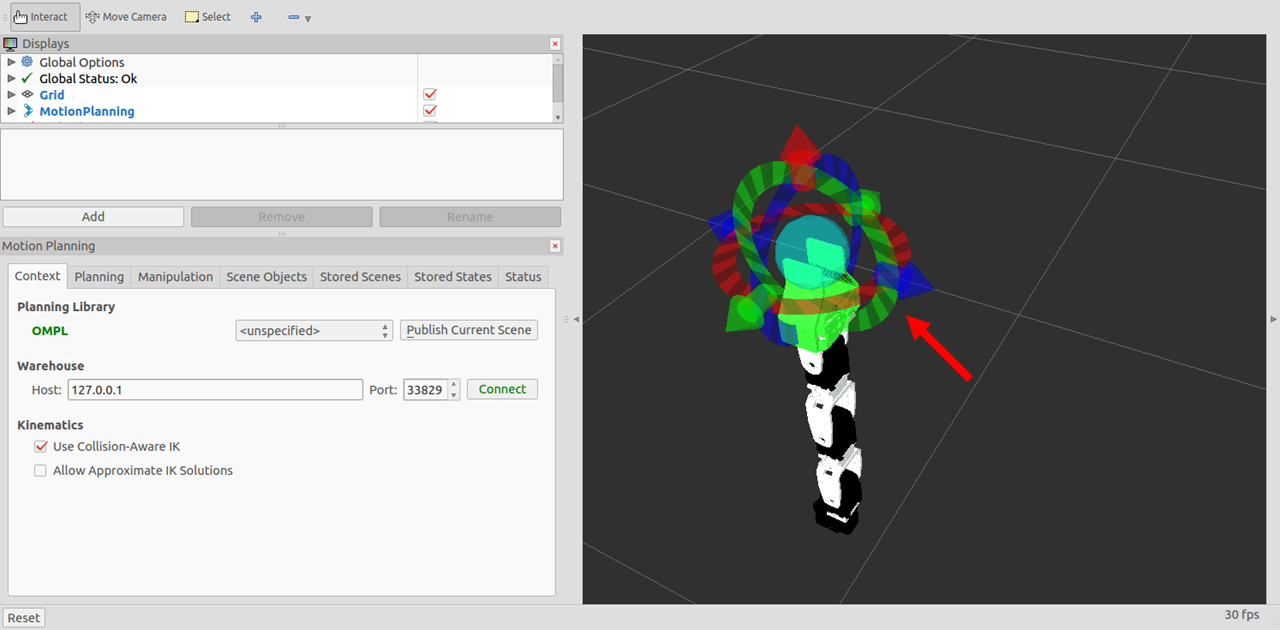
\includegraphics[width=12cm]{pictures/chapter11/pic_11_33.png}
  \caption{ロボットモデルとインタラクティブマーカー}
\end{figure}

実際に動作テストをしてみよう。まず緑色のボールをマウスで選択し、図11-34に示すように適当な場所に移動させる。ただし、ロボットアームが到達できない作業空間の外にボールを配置してしまうと、逆運動学の解を見つけることができない。ロボットアームを動作させるには、ボールは必ず作業空間内に配置する必要がある。

\begin{figure}[htp]
  \centering
  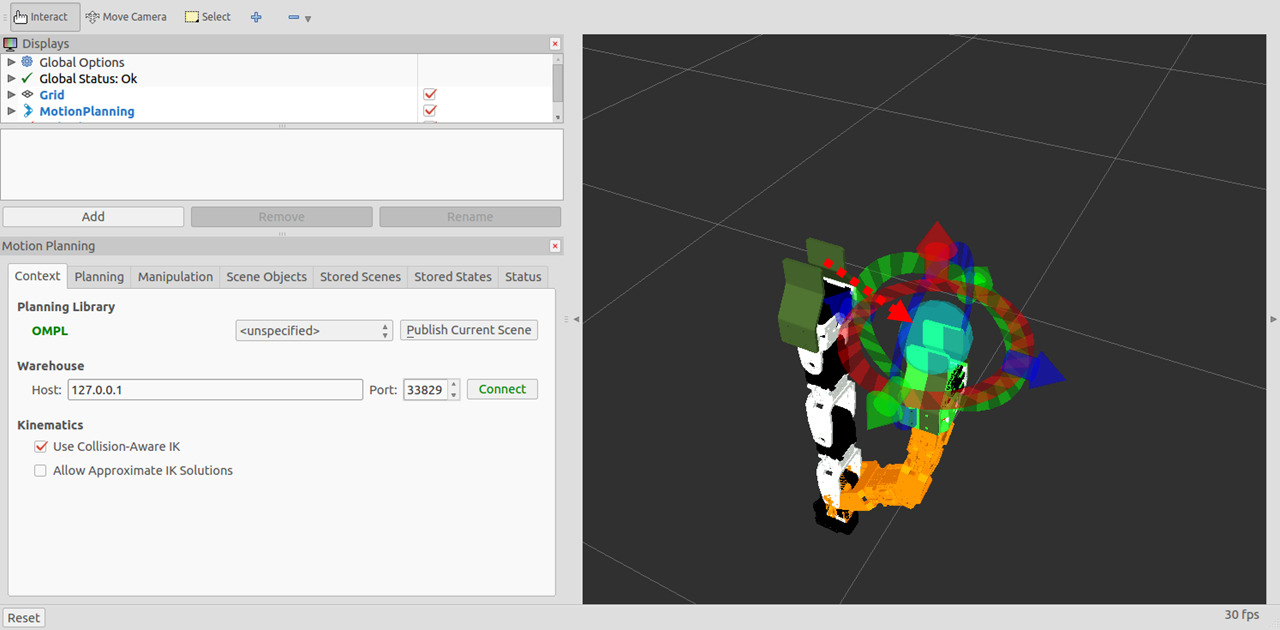
\includegraphics[width=12cm]{pictures/chapter11/pic_11_34.png}
  \caption{シミュレーション結果}
\end{figure}

ボールを目的の場所に移動させた後、RVizの左下のGUIパネルでPlanningタブを選択する。そしてCommandsの<Plan&Execute>ボタンをクリックすれば、図11-35のように、ボールの位置を目標にロボットアームが動作する。さらに、図11-36のようにRVizの左上にDisplaysパネルでMotionPlanning項目のPlanned Pathの[Show Trail]チェックボックスをチェックすると、ロボットアームの移動軌跡が確認できる。また、[Loop Animation]チェックボックスをチェックすると、アニメーションで動作を確認することもできる。

\begin{figure}[htp]
  \centering
  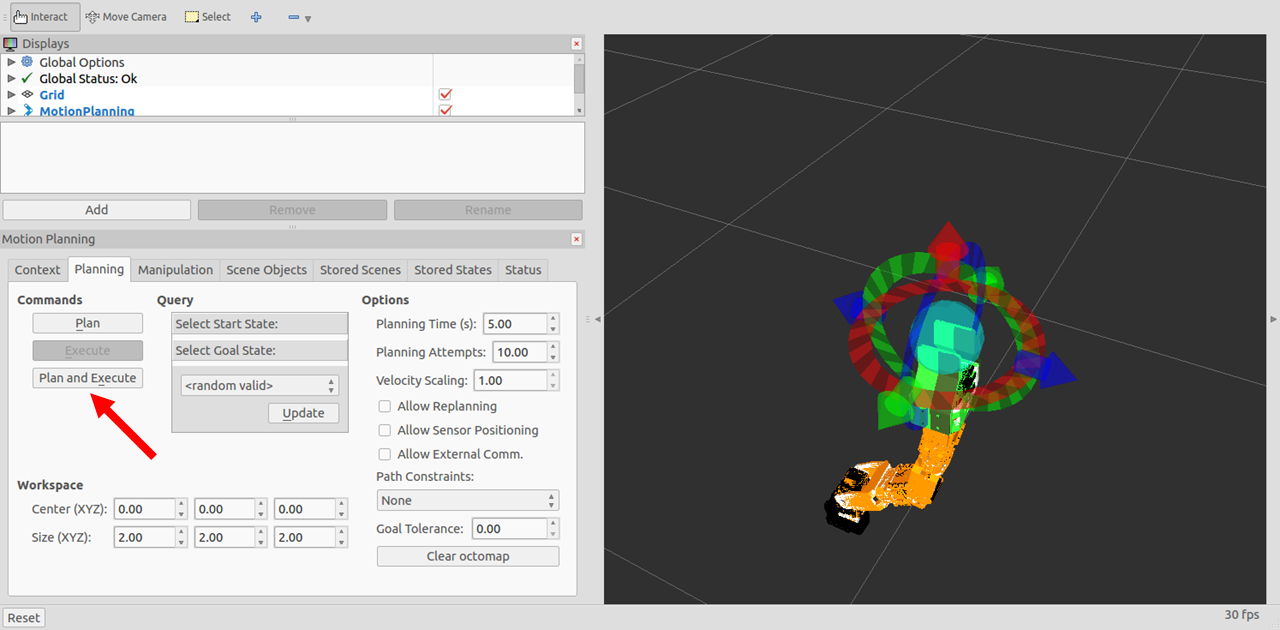
\includegraphics[width=12cm]{pictures/chapter11/pic_11_35.png}
  \caption{ロボットアームの把持動作}
\end{figure}

\begin{figure}[htp]
  \centering
  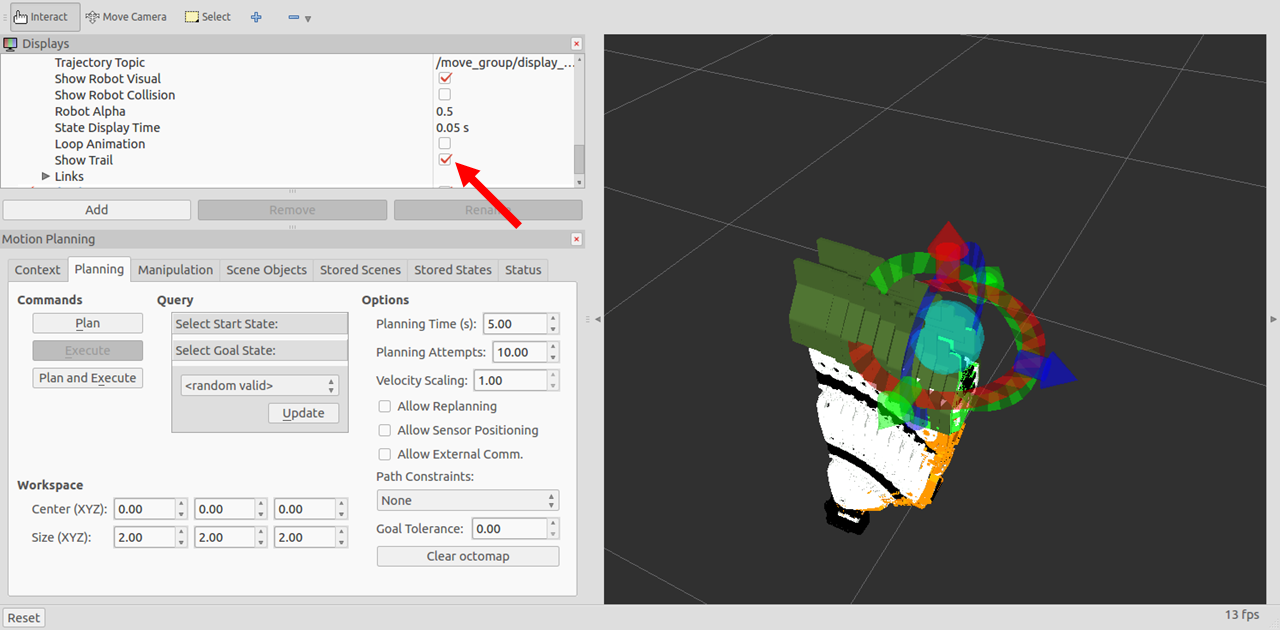
\includegraphics[width=12cm]{pictures/chapter11/pic_11_36.png}
  \caption{把持動作のアニメーション}
\end{figure}

%-------------------------------------------------------------------------------
\subsection{実際のロボットアームを使った動作確認}

本項では、実際にロボットアームを使ってMoveItの動作を確認してみる。まず、タートルボットアームを準備する。11.4.2項で述べたとおり、タートルボットアームは4つの関節と1つのグリッパーをもち、合計5つのアクチュエータで構成される。アクチュエータには、スマートアクチュエータ注12 DynamixelシリーズのAX-12A(図11-37)を使用している。PCでアクチュエータを直接制御するには、USB2Dynamixel(図11-38)をPCのUSBポートに接続して、制御コマンドをアクチュエータにシリアル通信で伝達する。

\begin{figure}[htp]
  \centering
  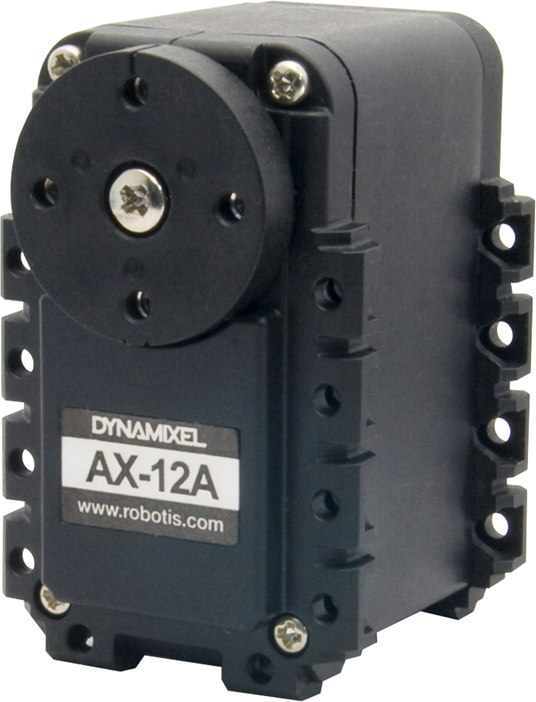
\includegraphics[width=4cm]{pictures/chapter11/pic_11_37.png}
  \caption{Dynamixel AX-12A}
\end{figure}

\begin{figure}[htp]
  \centering
  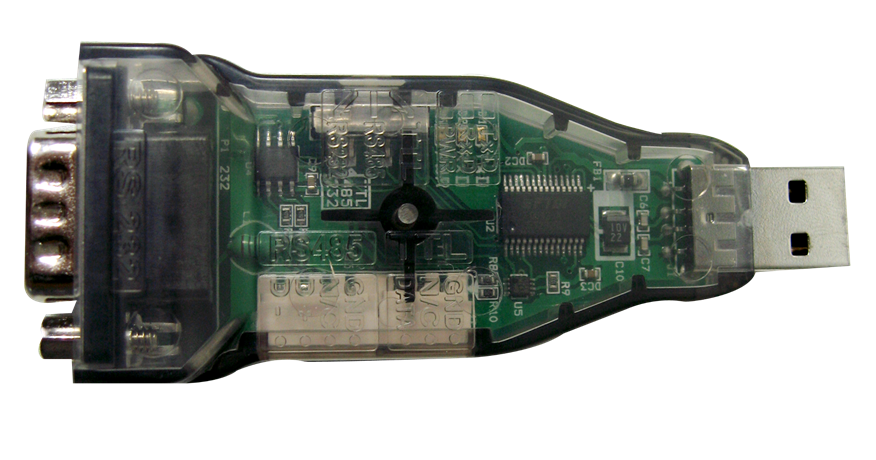
\includegraphics[width=6cm]{pictures/chapter11/pic_11_38.png}
  \caption{USB2Dynamixel}
\end{figure}

Dynamixelシリーズは、図11-39のようにデイジーチェーン(Daisy chain)方式(アクチュエータの信号線を直列に接続可能な方式)であり、配線が簡単になる。一つのアクチュエータは、モータ、減速ギア、コントローラ、駆動部、通信部で構成され、位置、温度、負荷、電圧などが出力できる。また、基本的な位置制御だけでなく、速度制御やトルク制御(一部のシリーズ)も可能である。
DynamixelシリーズのアクチュエータをROSで使用するには、dynamixelパッケージ注13かarbotixパッケージ注14のどちらかが必要になる。2つのパッケージのうち、タートルボットではarbotixのみをサポートしているので、ここではarbotixパッケージをインストールする。

\begin{lstlisting}[language=ROS]
$ sudo apt-get install ros-indigo-arbotix*
\end{lstlisting}

なお、参考までにdynamixelパッケージのインストール方法を以下に示す。

\begin{lstlisting}[language=ROS]
$ sudo apt-get install ros-indigo-dynamixel*
\end{lstlisting}

\begin{figure}[htp]
  \centering
  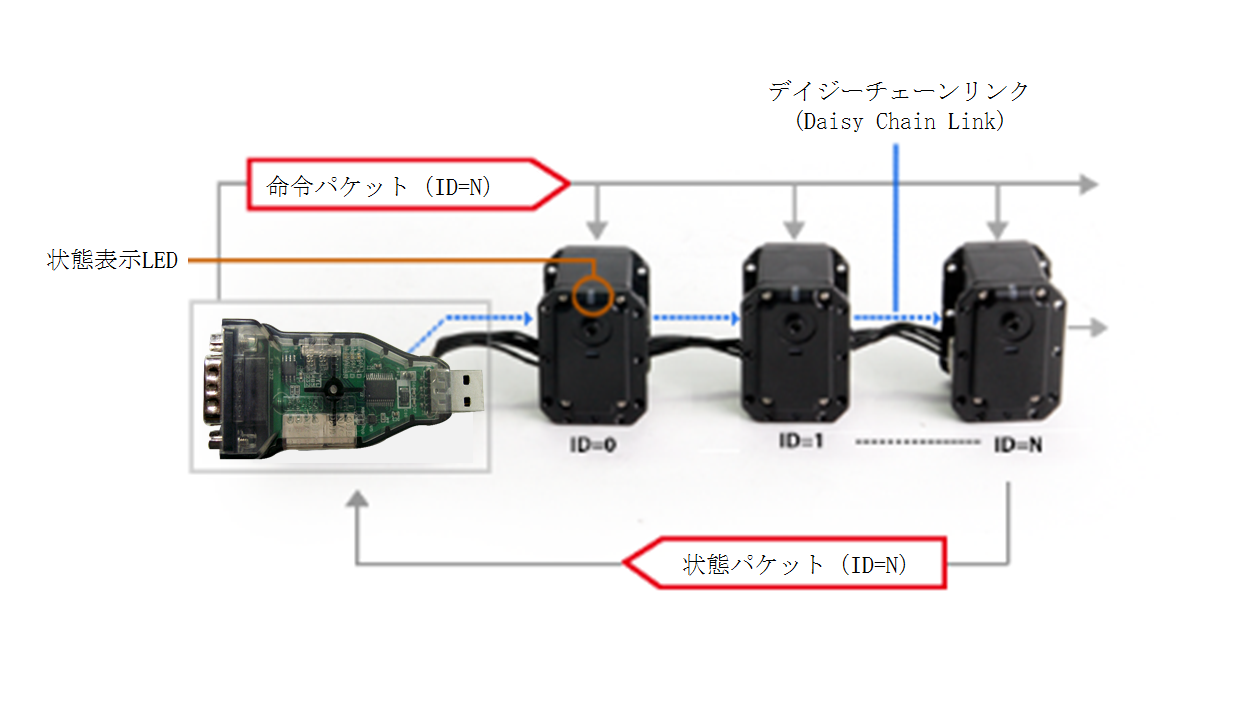
\includegraphics[width=12cm]{pictures/chapter11/pic_11_39.png}
  \caption{デイジーチェーン接続で複数のアクチュエータを制御}
\end{figure}

\subsubsection{手動制御による動作確認}

実際のロボットを使ってMoveItを実行する前に、タートルボットアームの各アクチュエータが正常に動作するかを確認する。まず、図11-38のUSB2Dynamixel\\をPCのUSBポートに挿入して、次のように、/devのなかで、どのポート番号で認識されるかを確認する。USBポートに他のシリアルデバイスが接続されていない場合は「ttyUSB0」として認識され、他のシリアルデバイスを使用している場合は他の名前で認識される。

\begin{lstlisting}[language=ROS]
$ cd /dev/
$ ls
autofs fb0z psaux ram4 sda5 tty0 tty21 tty34 tty47 tty6 ttyS13 ttyS26 uinput vcsa3
...
block fd ptmx ram5 sda6 tty1 tty22 tty35 tty48 tty60 ttyS14 ttyS27 ttyUSB0 vcsa4
...
ecryptfs ppp ram3 sda3 tty tty20 tty33 tty46 tty59 ttyS12 ttyS25 uhid vcsa2
...
$ sudo chmod a+rw /dev/ttyUSB0
\end{lstlisting}

ポート番号を確認したら、turtlebot\_arm\_bringupパッケージのconfigフォルダに移動し、arm.yamlファイルをエディタで開く。

\begin{lstlisting}[language=ROS]
$ roscd turtlebot_arm_bringup
$ cd config
$ gedit arm.yaml
\end{lstlisting}

arm.yamlファイルには、次のように、ポートの設定、スマートアクチュエータの読み取り/書き込みのサイクル、各関節の規定値が記載されている。ここで、「port:/dev/ttyUSB1」と書かれた太字の部分を、先に調べたポート番号(本書では「port:/dev/ttyUSB0」)に変更する。

\textbf{ファイル名:turtlebot\_arm/turtlebot\_arm\_bringup/config/arm.yaml}
\begin{lstlisting}[language=YAML]
port: /dev/ttyUSB1
read_rate: 15
write_rate: 25
joints: {
  arm_shoulder_pan_joint: {id: 1, neutral: 205, max_angle: 180, min_angle: -60, max_speed: 90},
  arm_shoulder_lift_joint: {id: 2, max_angle: 150, min_angle: -150, max_speed: 90},
  arm_elbow_flex_joint: {id: 3, max_angle: 150, min_angle: -150, max_speed: 90},
  arm_wrist_flex_joint: {id: 4, max_angle: 100, min_angle: -100, max_speed: 90},
  gripper_joint: {id: 5, max_speed: 90},
}
controllers: {
  arm_controller: {type: follow_controller, joints: [arm_shoulder_pan_joint, arm_shoulder_lift_joint, arm_elbow_flex_joint, arm_wrist_flex_joint], action_name: arm_controller/follow_joint_trajectory, onboard: False }
}
\end{lstlisting}

次に、PCに接続したUSB2Dynamixelにタートルボットアームを接続する。タートルボットアームの電源を入れ、arbotix\_guiを起動すると、図11-40の画面が表示される。画面右側のMove Servosタブに、5つの関節の項目が表示される。それぞれの関節のOn/Offをチェックボックスで選択でき、スライドバーで関節を動かすことができる。図11-40のように、すべてのチェックボックスを選択し、スライドバーを操作して、実際のロボットを動かしてみよう。ここまで問題がなければ、実際にロボットが動作するはずである。

\begin{lstlisting}[language=ROS]
$ roslaunch turtlebot_arm_bringup arm.launch --screen
$ arbotix_gui
\end{lstlisting}

\begin{figure}[htp]
  \centering
  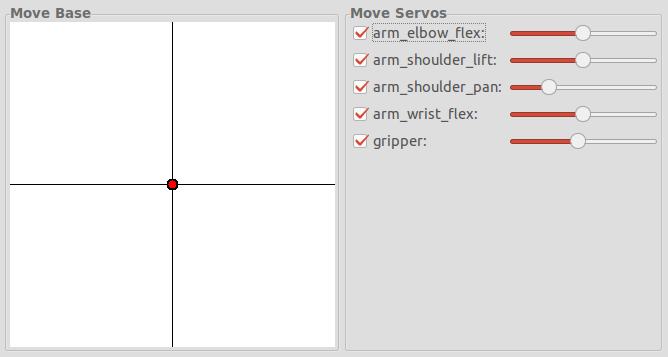
\includegraphics[width=12cm]{pictures/chapter11/pic_11_40.png}
  \caption{arbotix\_guiの操作画面}
\end{figure}

\subsubsection{MoveItを用いた実際のタートルボットの制御}

最後にMoveItを用い、実際のタートルボットを制御してみよう。ハードウェアの構成は上で説明した手動制御の場合と同じだが、実行するノードが異なる。今回は次のようにturtlebot\_arm\_bringupパッケージのarm.launchを起動する。またMoveItを起動するために、turtlebot\_arm\_moveit\_configパッケージのturtlebot\_arm\_moveit.launchを実行する。ここで11.5.3項ではオプションを付けずにturtlebot\_arm\_moveit.launchを実行し、仮想的にMoveItを動作させたが、今回は「sim:=false」として実際のロボットを制御する。

\begin{lstlisting}[language=ROS]
$ roslaunch turtlebot_arm_bringup arm.launch --screen
$ roslaunch turtlebot_arm_moveit_config turtlebot_arm_moveit.launch sim:=false --screen
\end{lstlisting}

RVizでのタートルボットアームの姿勢設定方法は、11.5.3項と同様である。緑色のボールをマウスで移動させると、図11-41に示すように、RViz画面内でタートルボットアームの関節が動いてアームの先がボールに向かって移動する。また<Plan and Execute>ボタンを押すと、実際のタートルボットアームが動作する。

\begin{figure}[htp]
  \centering
  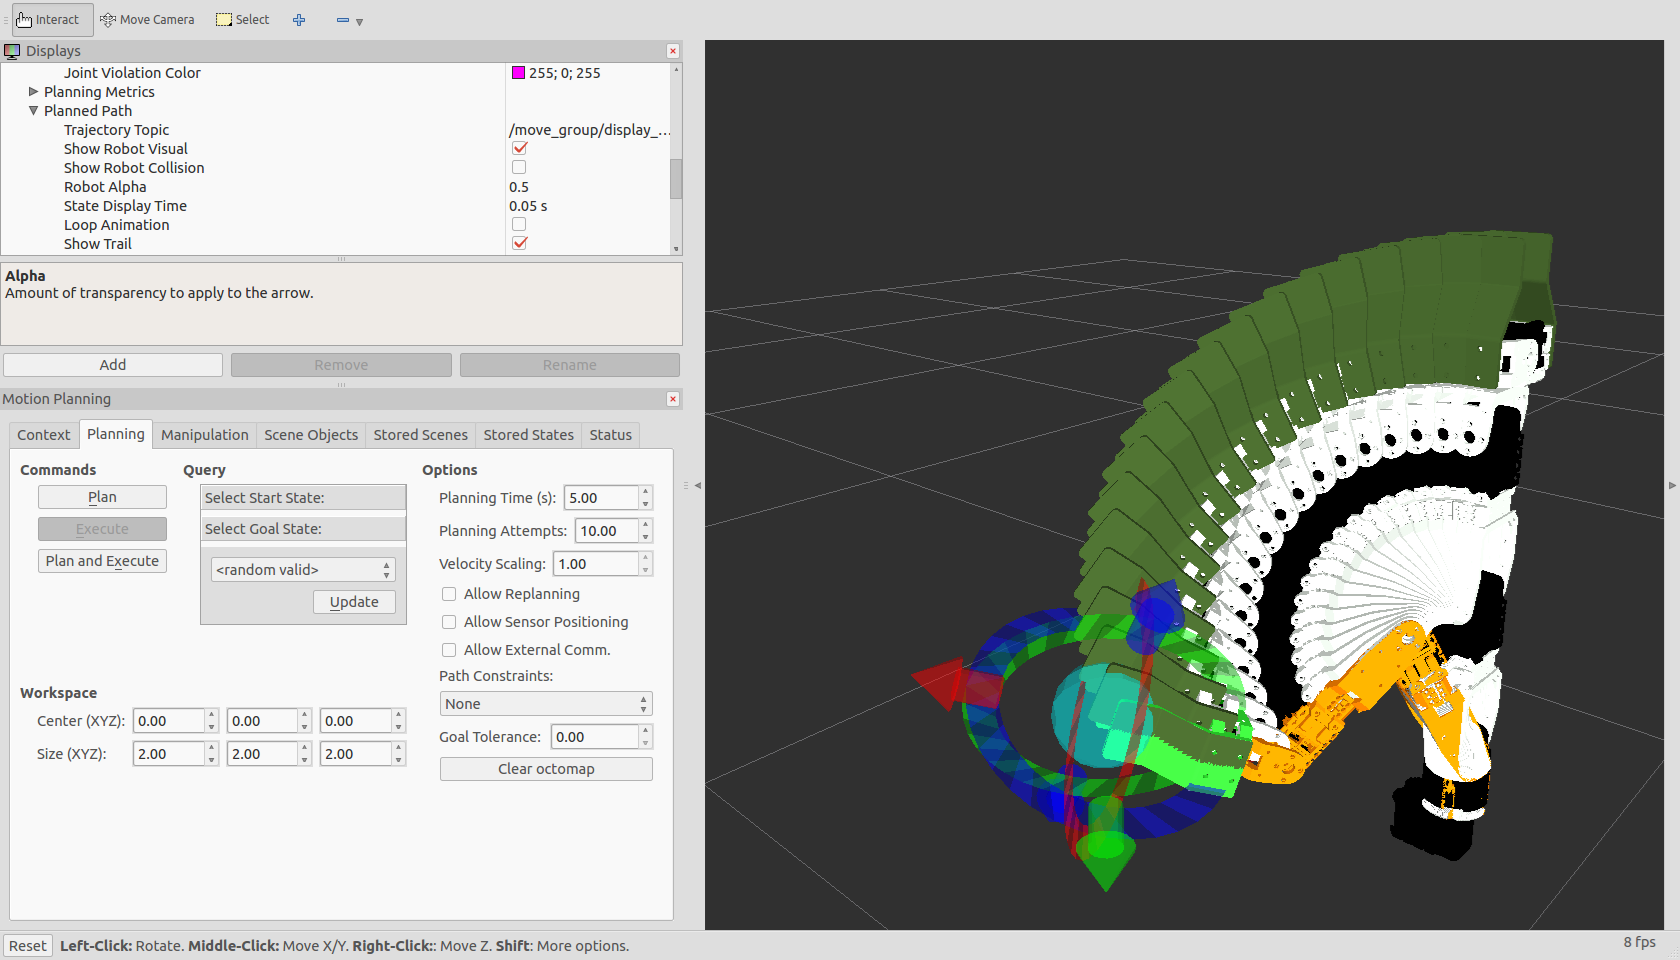
\includegraphics[width=12cm]{pictures/chapter11/pic_11_41.png}
  \caption{タートルボットアームが目標に向かって移動する様子}
\end{figure}

%-------------------------------------------------------------------------------
\section{タートルボットとタートルボットアーム}\index{タートルボットとタートルボットアーム}

最後に、9章で説明したタートルボットと、本章で説明したタートルボットアームを連携させる方法について説明する。タートルボットとタートルボットアームのモデルがそれぞれのパッケージに分かれているので、これらを一つに統合しなければならない。ここでは、タートルボットのモデルにタートルボットアームのモデルを追加する。次のようにturtlebot\_descriptionパッケージのrobotsフォルダに移動すると、kobuki\_hexagons\_kinect.urdf.xacroがある。

\begin{lstlisting}[language=ROS]
$ roscd turtlebot_description
$ cd robots/
$ sudo gedit kobuki_hexagons_kinect.urdf.xacro
\end{lstlisting}

このファイルはタートルボットのモデルを記述したものである。エディタで、これに次の太字部分を追加する。

\textbf{ファイル名:/opt/ros/indigo/share/turtlebot\_description/robots/kobuki\_hexagons\_ki\\nect.urdf.xacro}
\begin{lstlisting}[language=XML]
<?xml version="1.0"?>
<!--
- Base  : kobuki
- Stacks  : hexagons
- 3d Sensor : kinect
-->
<robot name="turtlebot" xmlns:xacro="http://ros.org/wiki/xacro">

  <xacro:include filename="$(find turtlebot_description)/urdf/turtlebot_library.urdf.xacro" />

  <include filename="$(find turtlebot_arm_description)/urdf/arm.xacro" />
  <turtlebot_arm parent="base_link" color="white" gripper_color="green" joints_vlimit="1.571" pan_llimit="-2.617" pan_ulimit="2.617">
    <origin xyz="0.12 0 0.42"/>
  </turtlebot_arm>

  <kobuki/>
  <stack_hexagons parent="base_link"/>
  <sensor_kinect  parent="base_link"/>
</robot>
\end{lstlisting}

次にRVizで仮想ロボットモデルを呼び出すと、図11-42のようにタートルボットとタートルボットアームが表示される。また、図11-43に示すように、Joint State PublisherのGUI画面で、タートルボットアームの各関節を操作できる。

\begin{lstlisting}[language=ROS]
$ roslaunch turtlebot_rviz_launchers view_model.launch
\end{lstlisting}

\begin{figure}[htp]
  \centering
  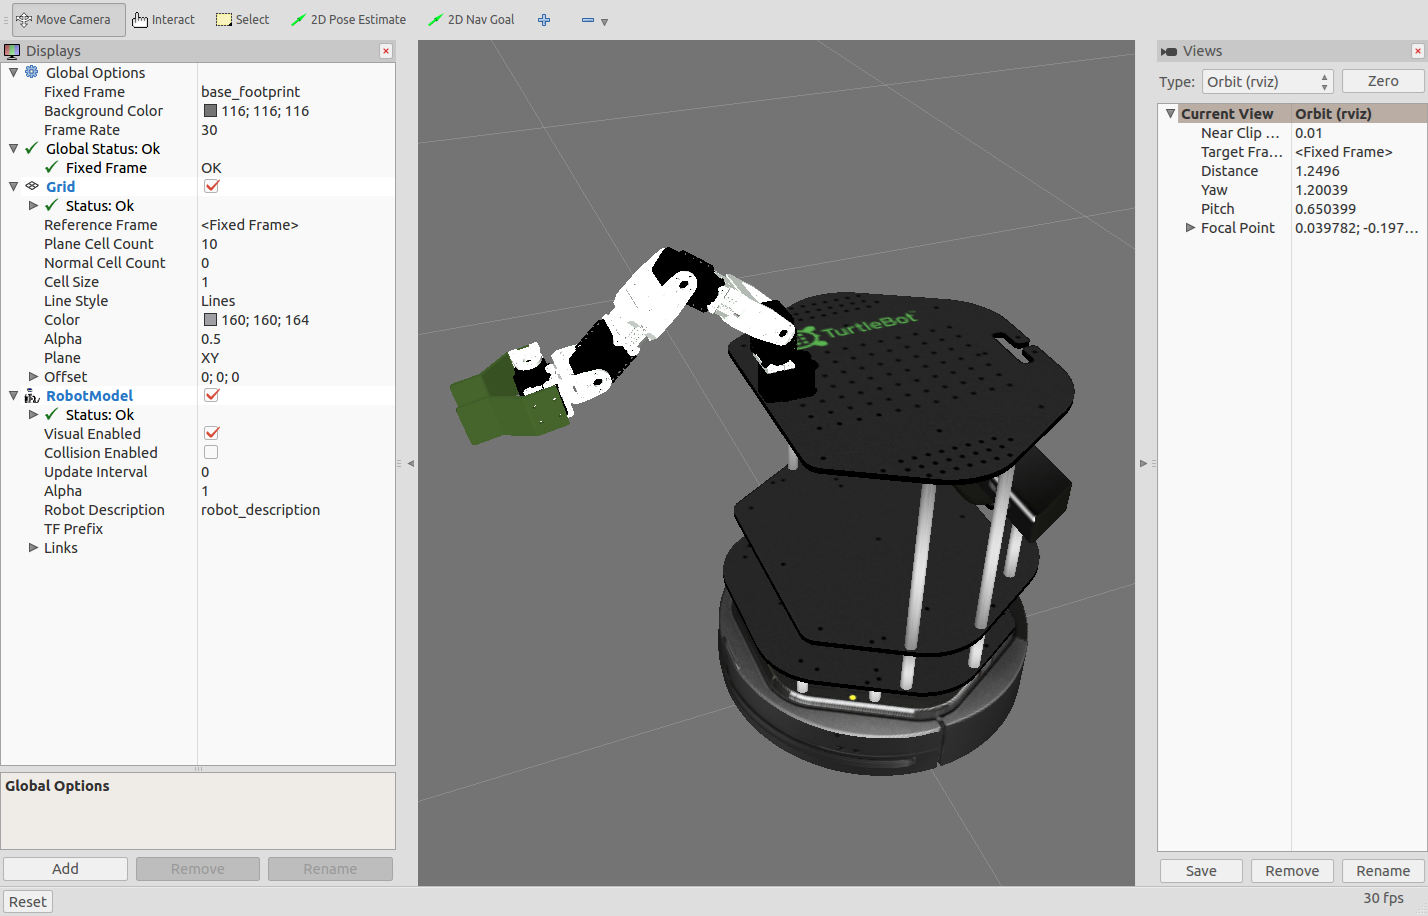
\includegraphics[width=12cm]{pictures/chapter11/pic_11_42.png}
  \caption{RVizで表示されたタートルボットとタートルボットアーム}
\end{figure}

\begin{figure}[htp]
  \centering
  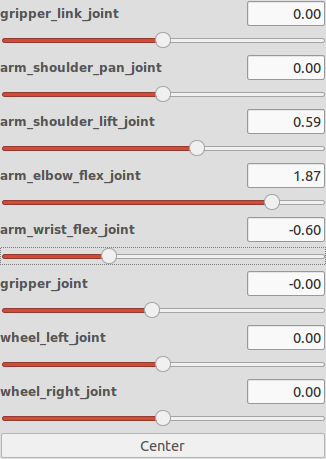
\includegraphics[width=6cm]{pictures/chapter11/pic_11_43.png}
  \caption{Joint State PublisherのGUI画面}
\end{figure}

% 注1  http://moveit.ros.org/
% 注2  http://wiki.ros.org/urdf
% 注3  http://wiki.ros.org/turtlebot_arm
% 注4  https://github.com/turtlebot/turtlebot_arm
% 注6  http://moveit.ros.org/robots/
% 注6  http://moveit.ros.org/documentation/concepts/
% 注7  http://wiki.ros.org/srdf
% 注8  http://moveit.ros.org/wiki/PR2/Setup_Assistant/Quick_Start
% 注9  http://www.orocos.org/kdl
% 注10 http://moveit.ros.org/wiki/Kinematics/IKFast
% 注11 http://wiki.ros.org/interactive_markers
% 注12 http://www.robotis.com/index/product.php?cate_code=131010
% 注13 http://wiki.ros.org/dynamixel_motor
% 注14 http://wiki.ros.org/arbotix

%-------------------------------------------------------------------------------
